\chapter{Performance Evaluation}
\label{chp:perfeval}

This chapter will focus on performance evaluation of credit mining system implementation in Tribler with both synthetic and real-world swarms. We start with simple and easy to understand experiments with predictable outcomes to validate the correctness of our work. Then we increase the complexity of our experiments in several steps towards evaluation within the real Internet environment. We will cover both the core components and proposed optimization. All the experiments in this chapter comply with the specifications mentioned in Section \ref{section:cmexp}. 

\section{Evaluation metrics}
\label{section:evalmetrics}
Throughout the experiments, we use several metrics to refer the credit mining system evaluation. In order to measure how many credit user already gain, \textit{Net upload gain}\cite{2015:creditmining:capota} is used. Net upload gain is defined as a difference between uploaded and downloaded bytes. To show how efficient a miner can get the credit after putting the investment, \textit{upload ratio} is also used. Upload ratio is the ratio between uploaded and downloaded bytes.

In order to measure whether miner consumes the resource efficiently, both maximum upload and download rate are considered. In most cases, maximum download rate and upload rate is 250 kB/s and 100 kB/s, respectively. We also combine this metric with how frequent a resource is used. For example, a miner that consumes 80\% of maximum upload rate for 70\% of its lifetime is using the resource more efficient than another one that only consumes the same amount for 50\% of its lifetime. A higher number of these metrics means that fewer resources are wasted. 

%We use average download speed in a specific period to measure user experience. However, observed download speed may look unstable because of \bt~nature. Therefore, as long as the measurement difference is not significant, we conclude that user will not experience noticeable performance drops. 

%community experience -> download speed average
\section{Validating the credit mining system}
\label{section:cmsvalidation}
The following experiments are specifically designed to be simple and able to validate all core components and algorithms of our credit mining research. All conditions are controlled and do not rely on external elements such as trackers or DHT. Our validation experiments test the basic swarm selection algorithm. The experiments will be conducted for one hour with 5 minutes swarm selection interval. 

\begin{figure}[h]
	\centering
	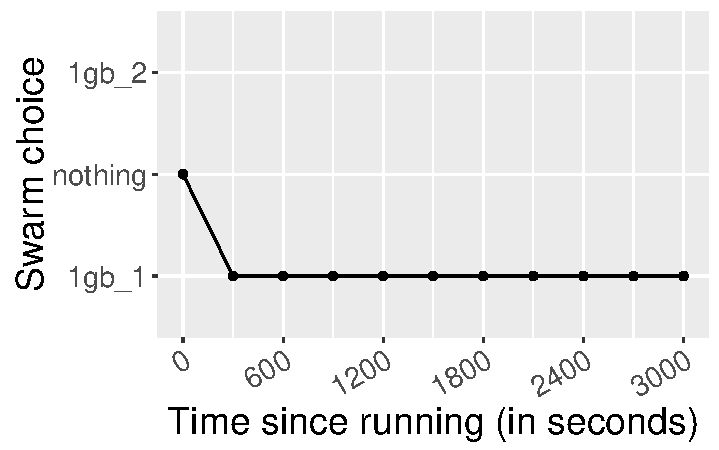
\includegraphics[width=0.5\textwidth]{pics/results/val0.pdf}
	\caption{Swarm selection in first experiment.}
	\label{fig:val0}
\end{figure}

In the first experiment, there are only two swarms: \texttt{1gb\_1} and \texttt{1gb\_2}. Swarm \texttt{1gb\_1} has one seeder, while \texttt{1gb\_2} has two. Both do not have any downloader. Swarms are distributed via \textit{channel} mechanism in Tribler. The miner then subscribed to this channel and get notified whether the swarms are added to the library. We expect the miner to choose swarm with the lowest number of seeder (\texttt{1gb\_1}). Figure \ref{fig:val0} shows the miner's swarm selection. The result is as expected. Although the miner already discovered the swarms in 10 seconds after it had started the system, it can only start mining in the next 5-minutes period. Therefore, in the first mining round, the miner could not choose anything because of lack of information.

\begin{figure}[h]
	\begin{subfigure}[t]{0.5\textwidth}
		\centering
		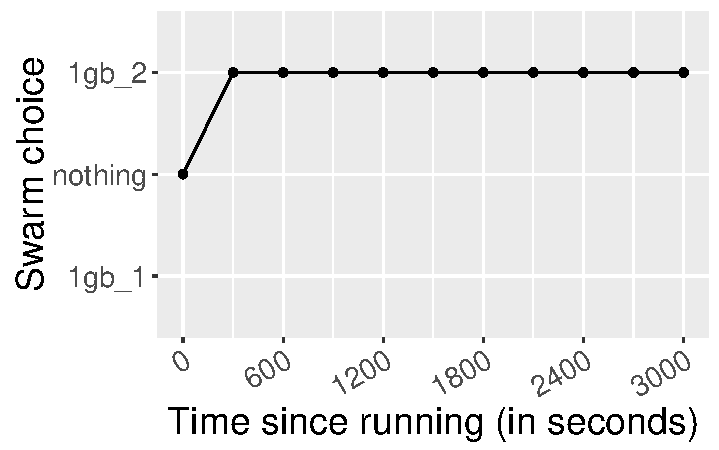
\includegraphics[width=\textwidth]{pics/results/valgain0.pdf}
		\caption{Swarm selection in second experiment.}
		\label{fig:val0gain}
	\end{subfigure}
	~
	\begin{subfigure}[t]{0.5\textwidth}
		\centering
		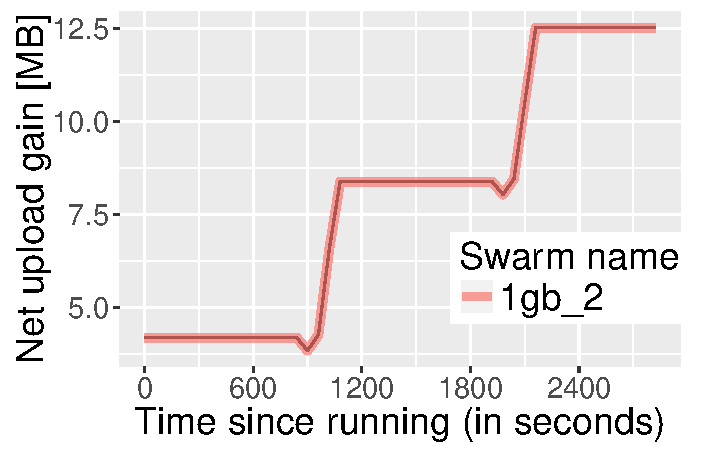
\includegraphics[width=\textwidth]{pics/results/valgain.pdf}
		\caption{Credit gained in second experiment.}
		\label{fig:vgain}
	\end{subfigure}
	\caption{Results for second experiment.}
\end{figure}

In our second experiment, we intend to run with a minimum number of downloaders. Both swarms now have one seeder. The number of downloaders is one for swarm \texttt{1gb\_1} and two  for \texttt{1gb\_2}. We expect the miner to select swarm with the higher number of downloaders (\texttt{1gb\_2}). In the meantime, the  gained credit and upload ratio will also be observed. The \texttt{share\_mode\_target} is set as one.

The result is again fit with our expectation. As shown in Figure \ref{fig:val0gain}, the miner correctly chooses undersupplied swarm (\texttt{1gb\_2}). Again, it starts mining after the second selection round. As for credit gain, as shown in Figure \ref{fig:vgain}, the miner get 12.5 MB with 1.99 as upload ratio. This upload ratio result is exceeding our target as specified in \texttt{share\_mode\_target}. 

\section{Prospecting hit experiment}
\label{section:prospectexp}
Key in prospecting is the ability to find a swarm that likely to give high investment return. In the following section, we will asses how well our prospecting algorithm can discard low-potential swarms on the Internet. Furthermore, we will also measure how fast and accurate the prospecting algorithm to find the high-potential swarms. 



\subsection{Filtering swarms on the Internet}
In the following experiment, we observe how the prospecting algorithm filters swarms on the Internet. The program uses a directory as a source. The \texttt{.torrent} files in the directory are collected by the crawler presented in Section \ref{section:predlsetup}. The result then will be compared to \textit{random} and \textit{sequential} method when fetching the rest of the pieces. Both methods are expected to filter less swarm than our method.

%To evaluate our approach, two different methods of finding pieces after the first piece has been downloaded are presented. Those are \textit{random} and \textit{sequential} piece finding. 

In this experiment, 1 swarm is inserted for every 7 seconds until the maximum amount of active swarm is reached. The number of maximum attempts to find rarest pieces is 60 times with 30 seconds interval. The number of piece that need to be downloaded is 4 pieces in 1 hour threshold. Swarm with small content size will be automatically discarded. We divide the failing result into four categories: \textit{timeout, zero peers, no information}, and \textit{no leecher}.

\textit{Timeout} is the condition where the threshold is reached, and the system could not finish the prospecting. \textit{Zero peers} happened when the system could not get any peers information. \textit{No information} means that there is not any piece information from known peers. In \textit{No leecher}, we could not find prospective downloaders so that made investment impractical. 

\begin{figure}[h]
	\centering
	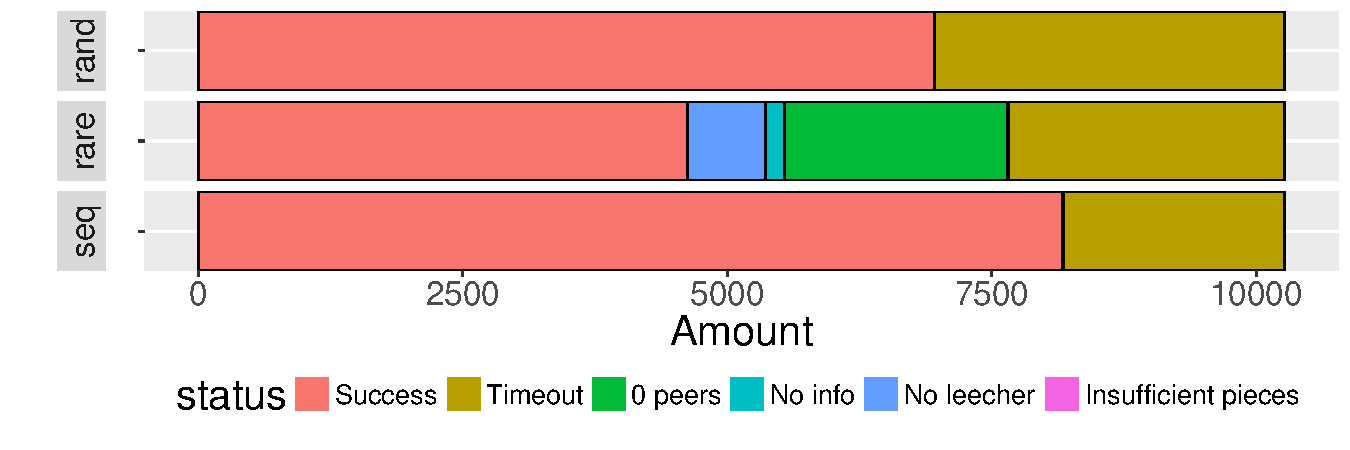
\includegraphics[width=\textwidth]{pics/results/dpredown_merge.pdf}
	\caption{Prospecting success percentage with three methods.}
	\label{fig:predownprecent}
\end{figure}

\begin{figure}[h]
	\centering
	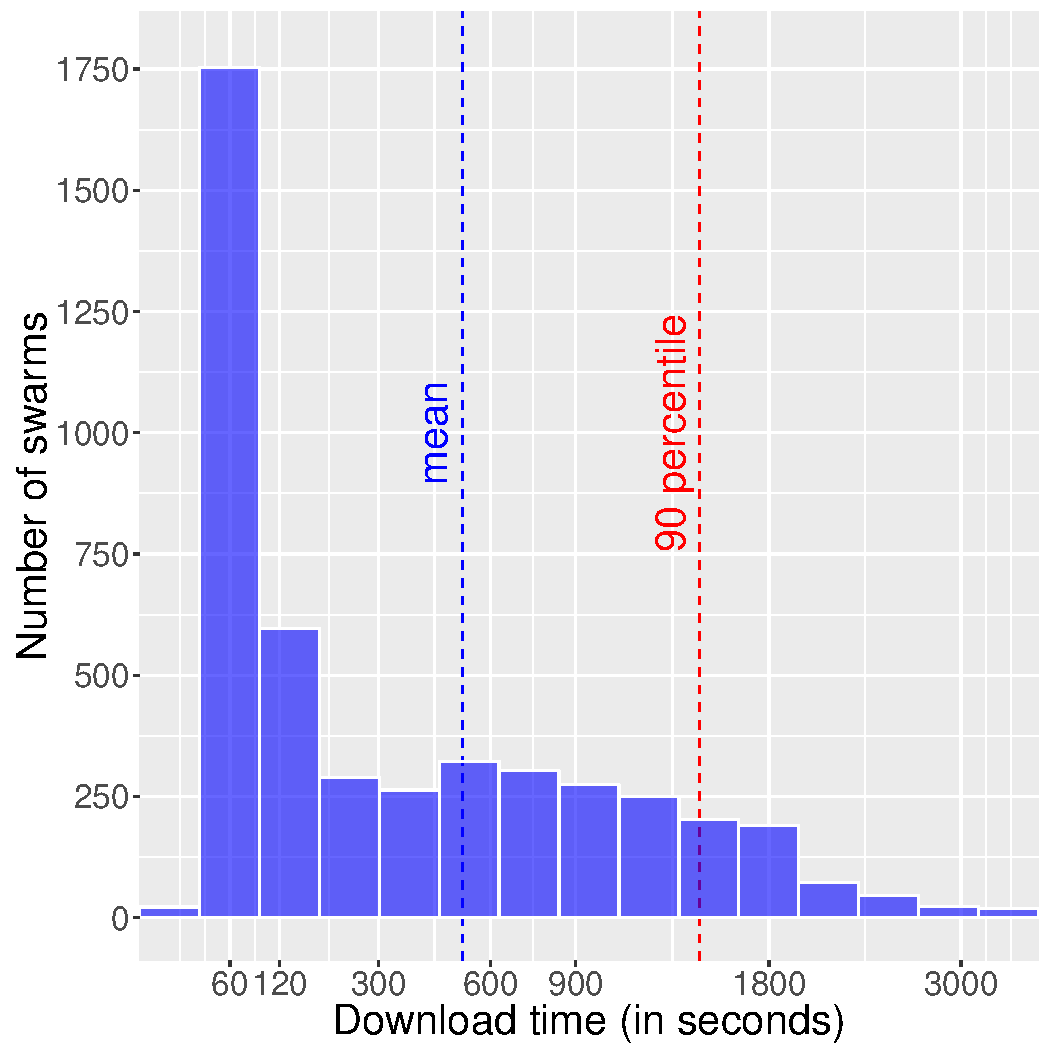
\includegraphics[width=0.6\textwidth]{pics/results/hpredown.pdf}
	\caption{Prospecting distributed time}
	\label{fig:predownhist}
\end{figure}

In the Figure \ref{fig:predownprecent}, it is shown the portion of swarm that has been successfully \textit{prospected}. Out of 13956 observed swarms, 3690 swarm has very small file size. This left us with 10266 swarms with 45\% finished, 25\% timed out, and 20\% with zero peers. Figure \ref{fig:predownhist} shows the distribution of time needed to download 4 of the rarest pieces on successfully prospected swarms (4623 swarms). Most of the swarms can be prospected in less than 2 minutes. The average time is 514 seconds, and 90\% percentile relies in 1440 seconds as shown in vertical blue and red line, respectively. By looking at this figure, the ideal threshold time should be around 30 minute instead of 60 minutes. We arrived at this conclusion because in less than 30 minutes, 90\% of successfully \textit{prospected} swarm is finished.

Now, we compare the result to both \textit{random} and \textit{sequential} method. Figure \ref{fig:predownprecent} shows that the number of swarm that is successfully prospected has significantly increased in both methods. Top and bottom part of the figure represents random and sequential method, respectively. Both approaches are resulting 0 for attempted failure swarm. This fact clarifies that most of the swarms in this experiment are alive. However, some of them do not have any downloader at the time of the experiment, thus made them inactive. The proposed method can safely discard those swarms as they are not suitable for investing. By discarding 54\% of the swarms, it filters 70\% and 160\% more than random and sequential method, respectively. Moreover, its behavior is in favor with \bt~piece policy. Just after finished prospecting, the upload ratio may be very high because the pieces we collected are prioritized to be uploaded like shown in the previous experiment.

\subsection{Finding undersupplied swarms}
In the following section, the speed and accuracy of prospecting algorithm to find undersupplied swarms will be evaluated. The experiments are conducted in a closed environment and have single community containing many swarms. Each swarm have 2 seeders and 1 downloader except for few swarms, which only have 1 seeder. We specify the number of undersupplied swarms as the percentage of all the swarm in the community. The maximum number of concurrent swarm for active prospecting is 30. The maximum number of active swarms for mining is the same as the number of expected undersupplied swarms. The experiments only consider seeder and leecher ratio in \textit{scoring} policy. Figure \ref{fig:timeprosexp} shows the time results with various portion of undersupplied swarms and community size. The black dot is the moment when miner discovers the swarm. Blue, red, and green line is the elapsed time for the miner to wait for prospecting, prospect, and mine, respectively.

\begin{figure}[th]
	\begin{adjustwidth}{-1.5cm}{}
	\begin{subfigure}[t]{0.6\textwidth}
		\centering
		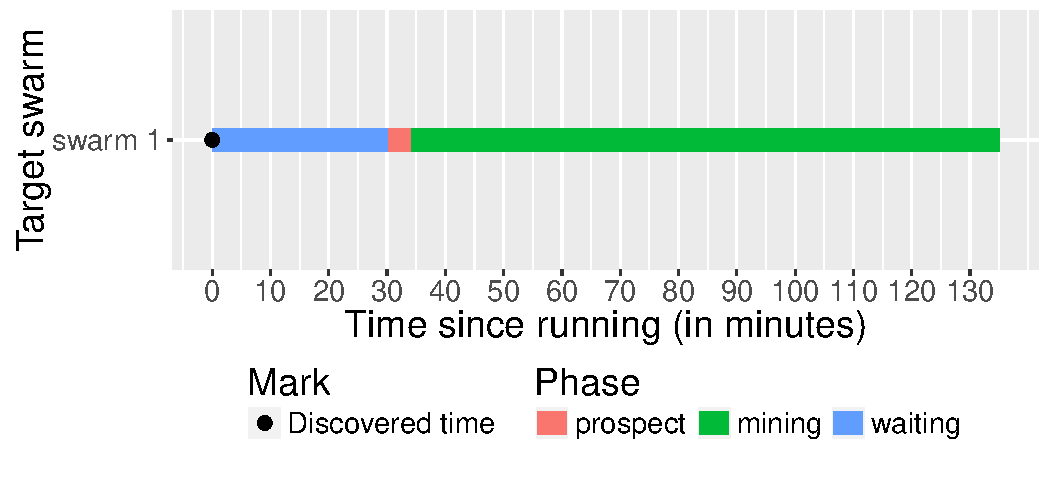
\includegraphics[width=\textwidth]{pics/results/time-1p100s.pdf}
		\caption{Investing timeline for 1\% of 100 swarm.}
		\label{fig:time1p100s}
	\end{subfigure}
	~
	\begin{subfigure}[t]{0.6\textwidth}
		\centering
		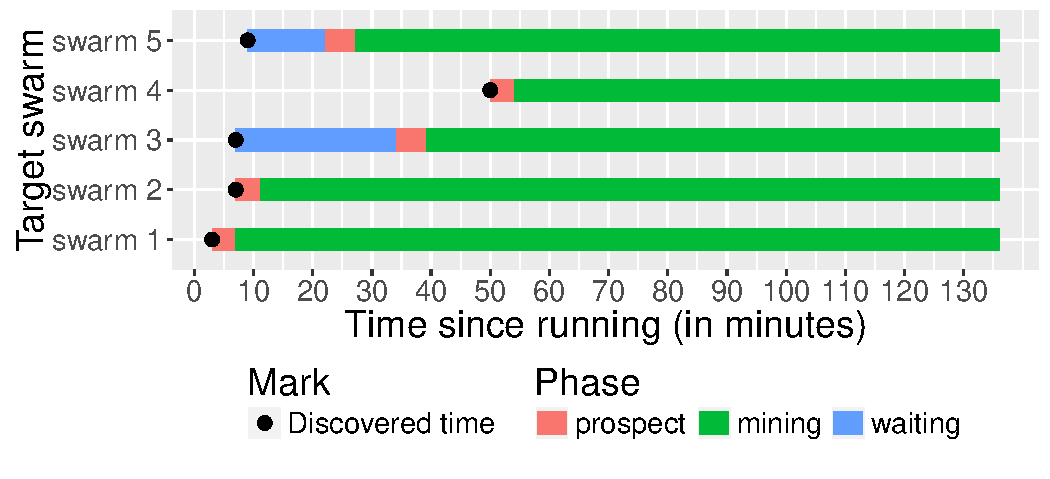
\includegraphics[width=\textwidth]{pics/results/time-5p100s.pdf}
		\caption{Investing timeline for 5\% of 100 swarm.}
		\label{fig:time5p100s}
	\end{subfigure}
	\begin{subfigure}[t]{0.6\textwidth}
		\centering
		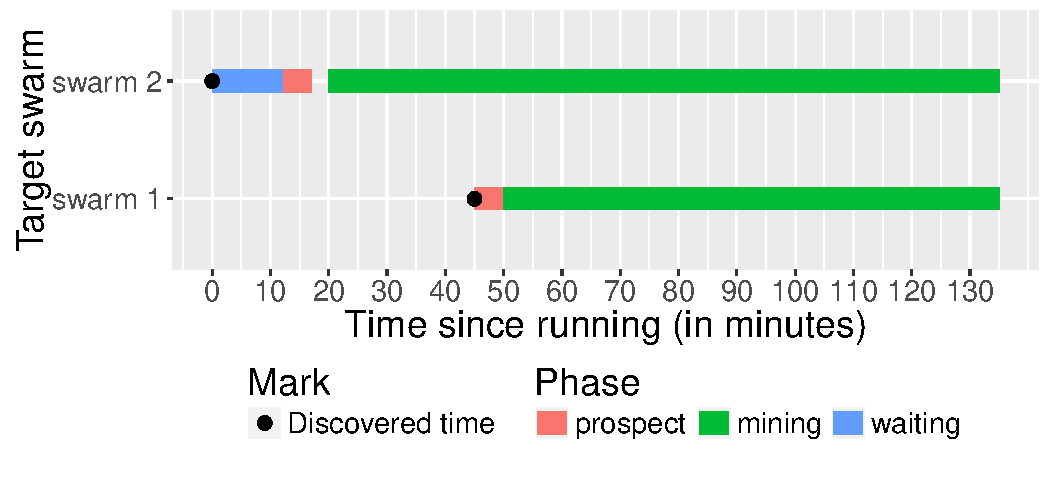
\includegraphics[width=\textwidth]{pics/results/time-1p200s.pdf}
		\caption{Investing timeline for 1\% of 200 swarm.}
		\label{fig:time1p200s}
	\end{subfigure}
	~
	\begin{subfigure}[t]{0.6\textwidth}
		\centering
		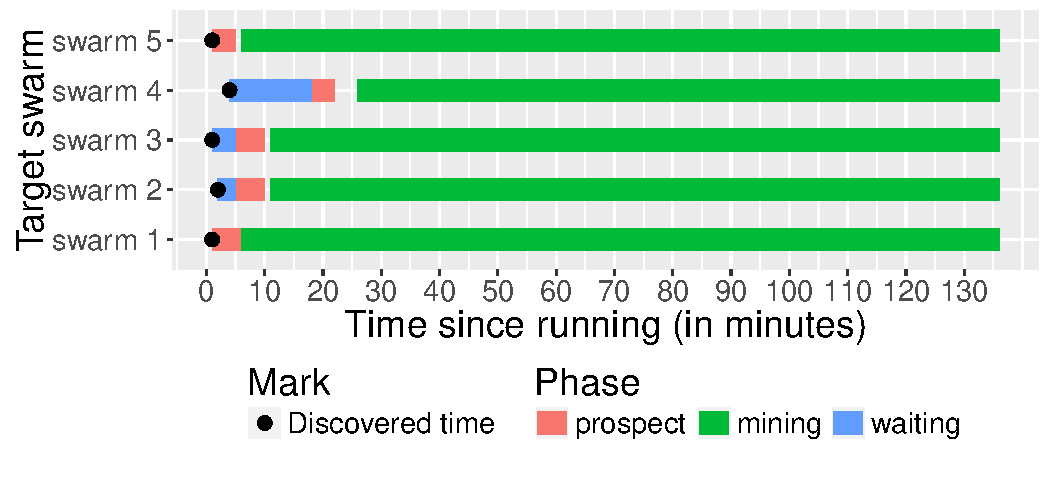
\includegraphics[width=\textwidth]{pics/results/time-25p200s.pdf}
		\caption{Investing timeline for 2.5\% of 200 swarm.}
		\label{fig:time2p200s}
	\end{subfigure}
	\caption{Investing timeline results.}
	\label{fig:timeprosexp}
\end{adjustwidth}
\end{figure}

The first experiment shown in Figure \ref{fig:time1p100s} has 1 undersupplied swarm (1\%) out of 100 swarms. The miner needs 34 minutes before it can start mining this swarm, mainly caused by waiting phase (88\%). The prospecting resulting an accurate swarm choice because in \textit{mining} phase, the miner continuously selects the targeted swarm until its downloader has finished downloading. In next experiment, the number of undersupplied swarm is increased to 5\% as its result shown in Figure \ref{fig:time5p100s}. Likewise, the prospecting accuracy is equally accurate. However, swarm waiting time and late discovery hold back the miner to mining all the targeted swarms. The average time of waiting and prospecting are 20 and 4.4 minutes, respectively. Moreover, \texttt{swarm4} was discovered very late on the 50th minutes.

Next, we changed the community size to 200. Figure \ref{fig:time1p200s} and Figure \ref{fig:time2p200s} shows the result for 1\% (2 swarms) and 5 swarms (2.5\%) for undersupplied swarm, respectively. For 5 underseeded swarms, the average prospecting time and waiting are 4.6 and 7 minutes, respectively. The \textit{mining} phase that starts regularly per 5 minutes causes the gap between \textit{prospecting} and \textit{mining} phase. The accuracy for this experiment is similar with the previous one. There is also a swarm that discovered very late which holds the miner to mine all the underseeded swarms.

From those results, we can conclude several insights. First, provided sufficient information, the prospecting algorithm is both fast and accurate. It only takes around 4-5 minutes and is much lower compared to both waiting and mining time. In general, its accuracy makes the \textit{mining} phase do not need to switch for other swarms. Second, waiting time and late discovery are the main causes that restrict miner to start mining all the undersupplied swarms as early as possible. Waiting time may be reduced by increasing maximum number of concurrent prospecting or by changing the prospecting queue system. Late discovery time is introduced by an external factor, which in this case, the swarm dissemination method by \textit{channel} in Tribler. 
%In one case, even some targeted swarms could not be discovered because of this problem. Ideally, swarms should be discovered regularly in short interval. 

\section{Evaluating Scoring policy}
\label{section:evalscoring}
In the following experiments, the \textit{mining} stage as part of our investing algorithm is evaluated. We focus on the \textit{scoring} policy that used in swarm selection. We wish to show that this policy selects the undersupplied swarms correctly. Furthermore, the mining performance from this selection will be evaluated. We will confirm that our policy will result a positive upload gain and ratio. 

The experiments run for three hours to compare \textit{scoring} and \textit{seederratio} policy. There are 10 swarms, and each has the same content size. Each swarm has a various number of seeders and fixed number of 5 downloaders. A single credit miner should select the underseeded swarms without relying on tracker or DHT. The credit mining system actively chooses at most 3 of those swarm to mine at a time. We set \texttt{share\_mode\_target} as 2. In the experiment, we use \textit{peer translation} function to interpret the number of seeder and leecher in a swarm. 

\subsection{The selected swarms}
In this section, we focus on what swarm the policy chooses. Two communities are presented. One is the community where there are a different number of seeder and leecher for all the swarms and with equal content size. Another one is the opposite, which is different content size with equal peers. \textit{Scoring} policy should perform equally with \textit{seederratio} policy in the first community. For the second community, the \textit{scoring} policy is expected to outperform \textit{seederratio} policy. We will specifically focus on the top three swarms that need to be seeded.

\label{section:chooseswarmexp}
\begin{figure}[h]
	\centering
	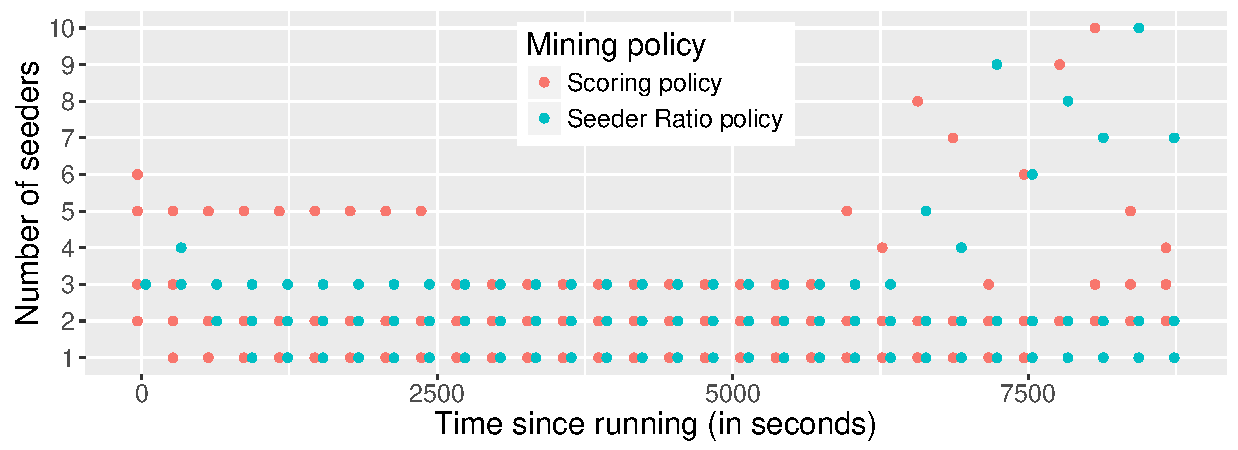
\includegraphics[width=\textwidth]{pics/results/scsr_notrig_scatter.pdf}
	\caption{Seeder ratio and scoring policy swarm selection.}
	\label{fig:scatterscsrnotrig}
\end{figure}

Regarding the first community, Figure \ref{fig:scatterscsrnotrig} shows which swarms the policies select. Focusing on the three targeted swarms, they are chosen for 79\% and 89\% for scoring policy and seeder ratio policy, respectively. At the beginning (timestep 0-2500), the lack of information causes peer translation function to be less accurate. However, as the time goes on, more information can be collected, swarm information is stabilized, and both policy and peer translation function become more accurate. When the current swarm is saturated, the effect is inverted. The information of other swarms become very outdated and cause both policy and peer translation function to have inaccurate result. The system has to rejoin other swarms to fetch the latest information. That explains the policy choice dispersion in the last 40 minute (2500 seconds) near the end. 

\begin{figure}[b!]
	\begin{adjustwidth}{-1.5cm}{}
		\begin{subfigure}[t]{0.6\textwidth}
			\centering
			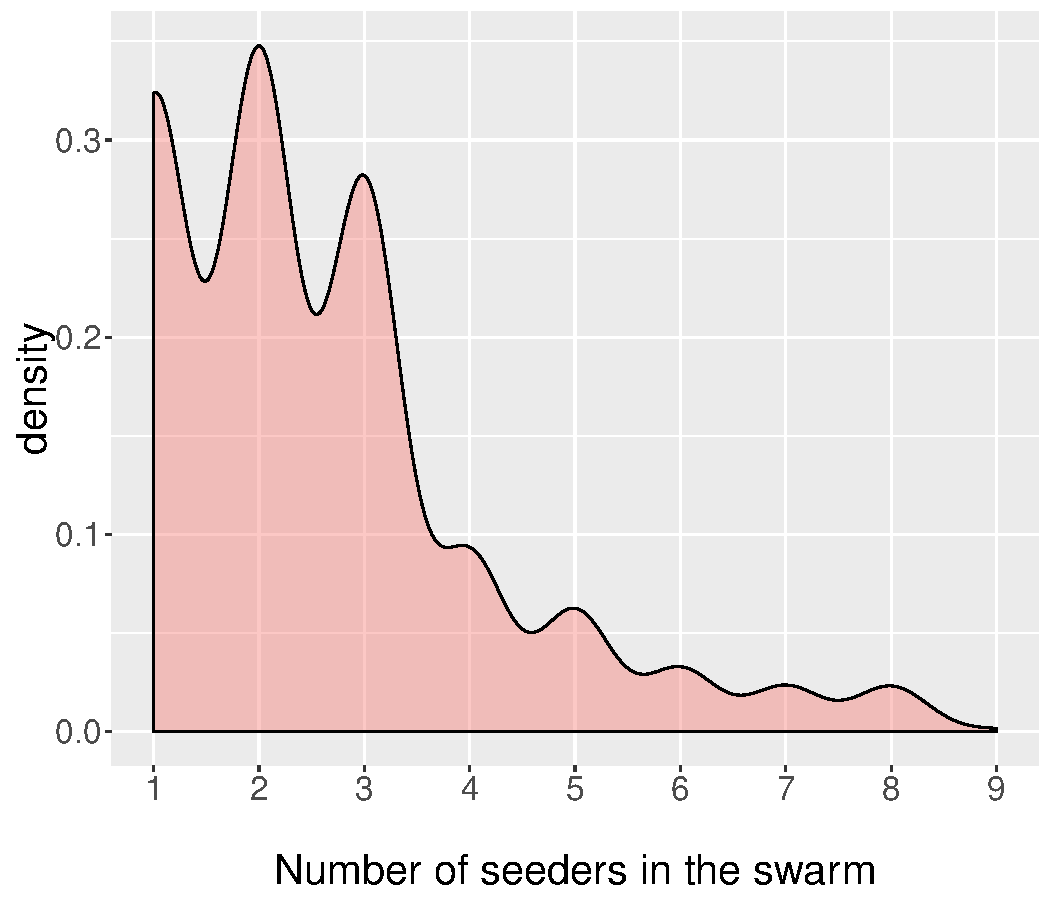
\includegraphics[width=\textwidth]{pics/results/sc10_density.pdf}
			\caption{Scoring ratio swarm selection with 10 miners.}
			\label{fig:scattersc10}
		\end{subfigure}
		~
		\begin{subfigure}[t]{0.6\textwidth}
			\centering
			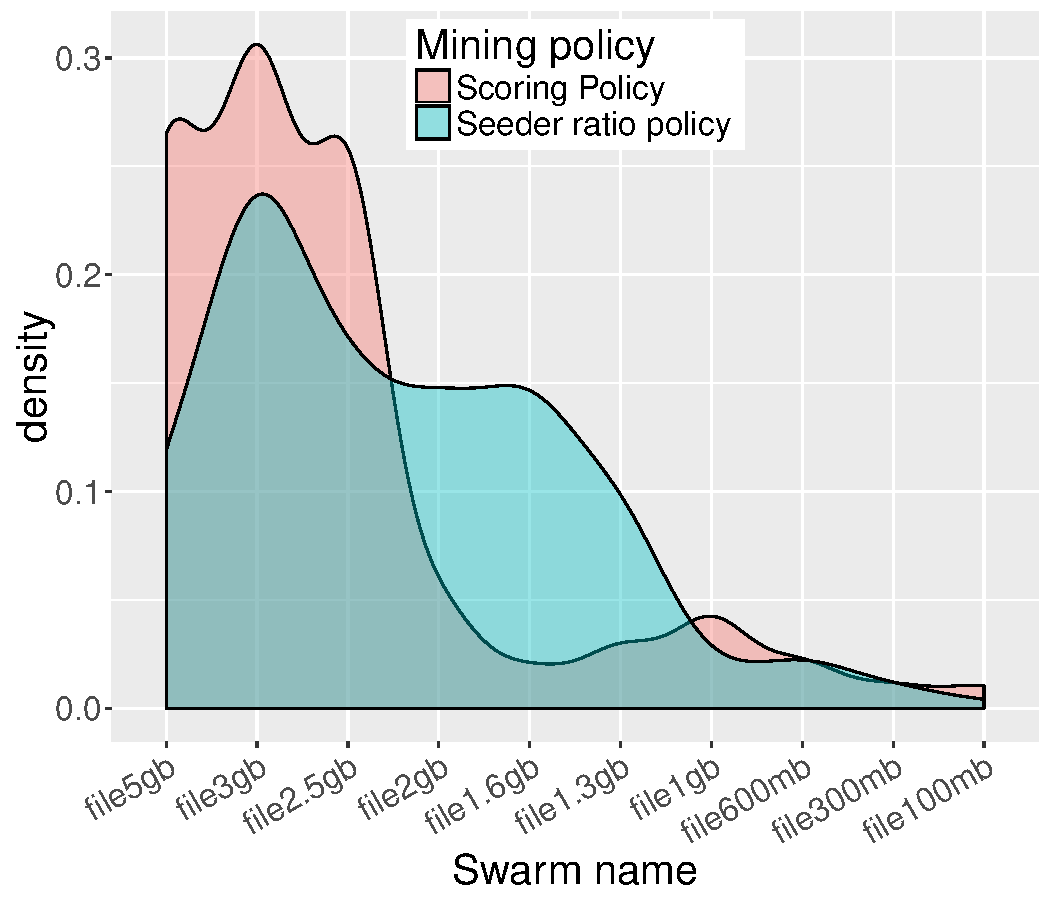
\includegraphics[width=\textwidth]{pics/results/scmulti_density.pdf}
			\caption{Swarm selection on swarms with different content size.}
			\label{fig:scatterscmulti}
		\end{subfigure}
		\caption{Swarm selection result on extended experiment.}
	\end{adjustwidth}
\end{figure}

The policy still valid when there are more than one miner in the community. To support this argument, we conducted a similar experiment with 10 credit miners with scoring policy. Shown in Figure \ref{fig:scattersc10}, the miners still choose the first three lowest-seeded swarm for the 80\% of the experiment. 

Figure \ref{fig:scatterscmulti} shows what the policies choose in the community with different file size among the swarms. For each policy, we conducted 3 experiments with only single miner each. From the result, scoring policy mainly chooses swarms with a large file. On the contrary, in seeder ratio, it frequently chooses other swarms as well. A swarm that has large files will have slower completion rate on its peers compared to one that has small files. Slower completion rate also means there are more rare pieces in a swarm, hence low piece availability. In this experiment, the target swarms are \texttt{file5gb}, \texttt{file3gb}, and \texttt{file2.5gb}. Scoring policy correctly detect the piece shortage problem and address it by choosing swarm with lowest piece availability. From the three targeted swarm, scoring policy chooses 82\%. On the other hand, seeder ratio sees all the swarm as equal, and the behavior is unpredictable. It chooses 67\% of the three targeted swarms.

\subsection{Obtained gain by the selection}
\label{section:resultgain}
The following results are presented to know the actual gain obtained as a result of swarm selection presented in the first community of Section \ref{section:chooseswarmexp}. Furthermore, we intend to know the swarm stimulation effect on credit gain. We expect the credit gain can be increased if it is still possible.

%By its nature, credit mining system only able to control what swarm to choose and how long the mining in one session is. After a swarm has been chosen, \textit{libtorrent} with its \textit{share mode} will do the rest. This causes slightly different results in each experiment. However, if the swarm selection constantly chooses a particular swarm, we expect the trend to be similar. 

\begin{figure}[h!]
	\begin{adjustwidth}{-1.5cm}{}
		\begin{subfigure}[t]{0.6\textwidth}
			\centering
			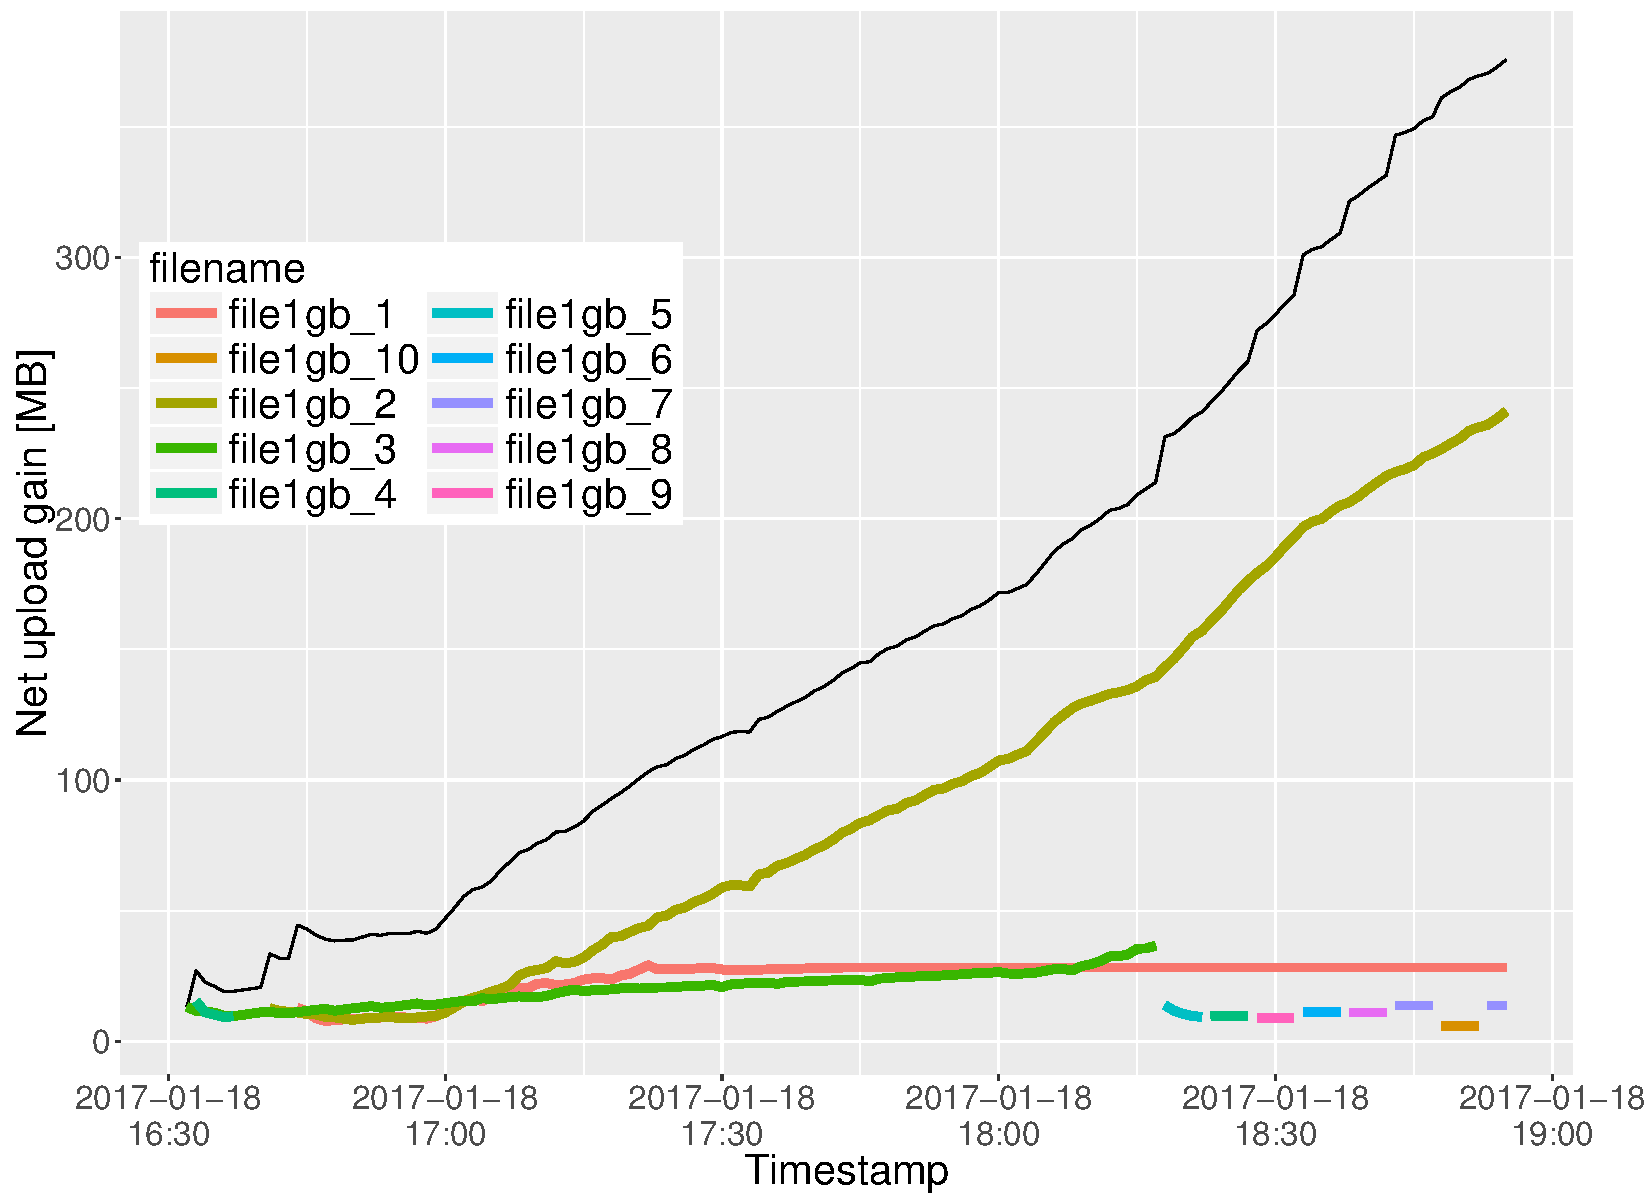
\includegraphics[width=\textwidth]{pics/results/simple1_sr_notrig.pdf}
			\caption{Seeder ratio policy gain.}
			\label{fig:simplesrnotrig}
		\end{subfigure}
		~
		\begin{subfigure}[t]{0.6\textwidth}
			\centering
			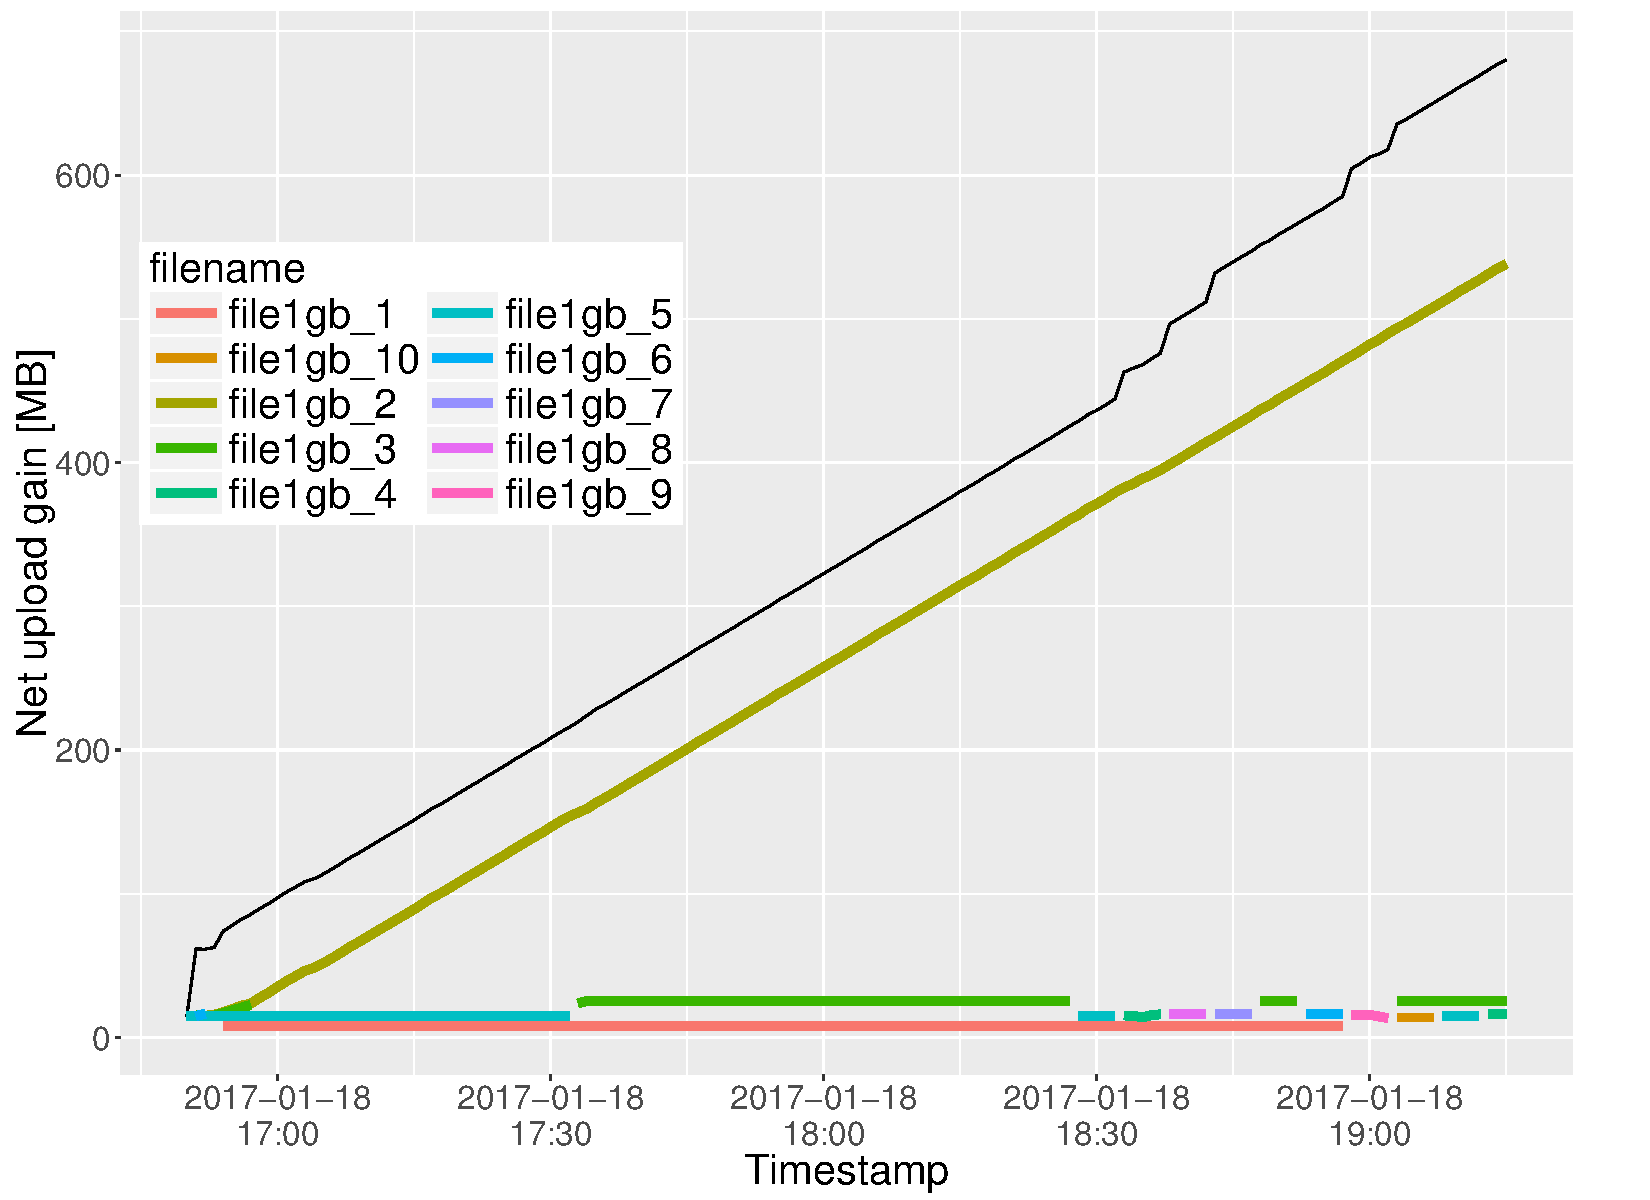
\includegraphics[width=\textwidth]{pics/results/simple1_scsr_notrig.pdf}
			\caption{Scoring policy gain.}
			\label{fig:simplescsrnotrig}
		\end{subfigure}
		\caption{Net upload gain of both policies.}
	\end{adjustwidth}
\end{figure} 

The obtained gain of applying seeder ratio policy is shown in Figure \ref{fig:simplesrnotrig}. A swarm with 2 seeders (\texttt{file1gb\_2}) is dominating the result. The rest of the selected swarms are relatively constant most of the time. Swarm \texttt{file1gb\_2} average seeding speed is 61 kB/s, which is more than half of the maximum speed on a single peer. This swarm also used a significant resource, which is more than 80\% of the maximum upload rate, for 44.67\% of its lifetime. At the end of the experiment, it reaches 241 MB gain and 2.005 upload ratio. As a comparison, the average upload ratio is 2.650.

In Figure \ref{fig:simplescsrnotrig}, scoring policy is applied. Unsurprisingly, the trend is similar. This time, the gain is 538 MB, almost twice as of the seeder policy with the same swarm.  Although \texttt{file1gb\_2} returned the highest gain, its upload ratio is not the highest by only 2.99.  The highest ratio is returned by \texttt{file1gb\_7} by 4.91, and the average from all the swarms is 3.718. Average upload speed for this swarm is 94.4 kB/s with 90\% of the observation is taking more than 80\% of the maximum upload rate. By this results, it is clear that the factor that limits credit mining system obtained higher gain is the maximum upload rate. 

After we observed those, we come to three conclusions. First, our hypothesis about the similar choice in this particular experiment on both of the policies is stand corrected. Although the gain is significantly different, it was not directly caused by the mining system. Instead, it is part of the \bt~protocol that builds up the download and upload speed. Second, although the resource may be used to its full capacity like shown in Figure \ref{fig:simplescsrnotrig}, it is entirely possible that it is not used efficiently. This is shown by the inactivity from the other swarms. Net upload gain for other swarms is barely increasing for both cases. This locked up condition is caused by the \textit{libtorrent}'s \textit{share mode} algorithm and its cause and possible solutions already discussed in Section \ref{section:sharemode}. Third, the swarm that gets the highest net upload gain does not necessarily have the highest ratio. We believe it is caused by the prospecting mechanism that downloads only a few rarest pieces and then uploads those pieces to most of the peers. After downloading rarest pieces, some of the swarms are not chosen by policy. Therefore, the ratio keeps high because there is not any downloading activity.

\subsubsection{The effect of stimulating swarms}
With swarm stimulation, inactive swarms tend to gain more credits when mined. Figure \ref{fig:simplesrtrig} shows the case for seeder ratio policy and Figure \ref{fig:simplescsrtrig} for scoring policy. We specifically focus on swarm \texttt{file1gb\_1} and \texttt{file1gb\_3} because they are the most affected swarm by stimulation mechanism. Table \ref{tbl:stimul} shows the stimulation effect of those swarms.

\begin{figure}[h]
	\begin{adjustwidth}{-1.5cm}{}
		\begin{subfigure}[t]{0.6\textwidth}
			\centering
			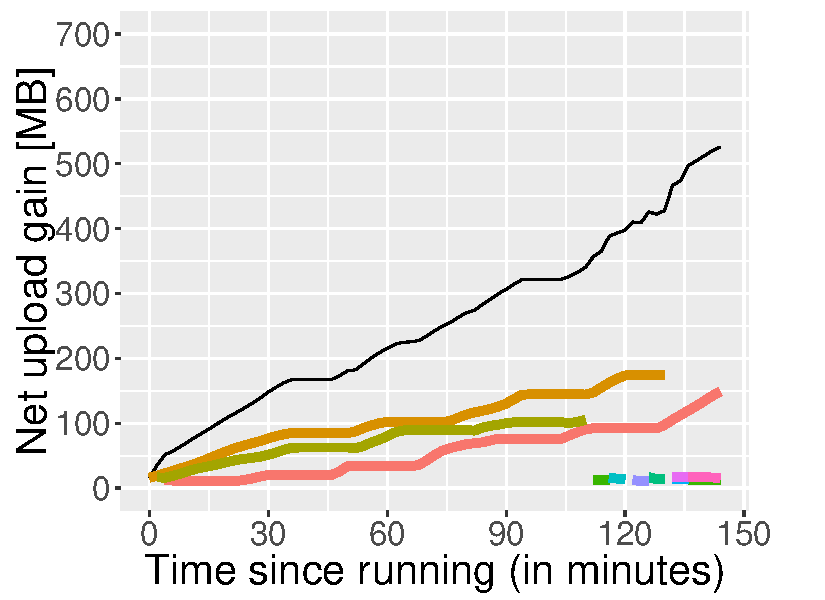
\includegraphics[width=\textwidth]{pics/results/simple3_sr_trig.pdf}
			\caption{Seeder ratio policy gain with stimulation enabled.}
			\label{fig:simplesrtrig}
		\end{subfigure}
		~
		\begin{subfigure}[t]{0.6\textwidth}
			\centering
			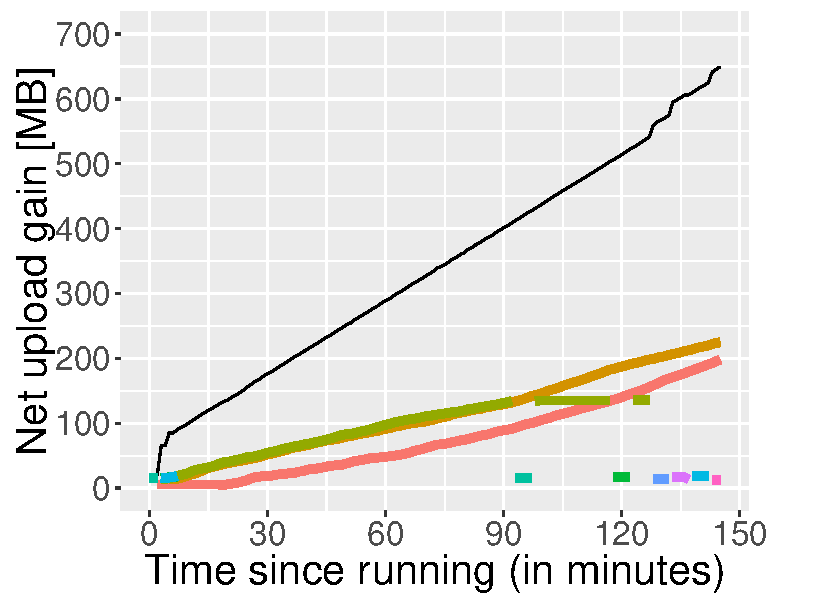
\includegraphics[width=\textwidth]{pics/results/simple1_scsr_trig.pdf}
			\caption{Scoring policy gain with stimulation enabled.}
			\label{fig:simplescsrtrig}
		\end{subfigure}
		\caption{Net upload gain of both policies with stimulation enabled.}
	\end{adjustwidth}
\end{figure}

\begin{table}[h]
	\centering
	\caption{Stimulation effect on gained credit.}
	\label{tbl:stimul}
	\begin{adjustwidth}{-1cm}{}
	\begin{tabular}{|c|c|l|l|l|l|}
		\hline
		\multirow{2}{*}{\textbf{Swarm name}} & \multirow{2}{*}{\textbf{Policy}} & \multicolumn{2}{c|}{\textbf{Upload ratio}} & \multicolumn{2}{c|}{\textbf{Net upload gain (in MB)}} \\ \cline{3-6} 
		&  & \textbf{St. Enabled} & \textbf{St. Disabled} & \textbf{St. Enabled} & \textbf{St. Disabled} \\ \hline
		\texttt{file1gb\_1} & Seeder ratio & 3.37 & 1.95 & 148 & 28 \\ \hline
		\texttt{file1gb\_3} & Seeder ratio & 2.88 & 1.95 & 105 & 26 \\ \hline
		\texttt{file1gb\_1} & Scoring & 3.07 & 2.84 & 198 & 77 \\ \hline
		\texttt{file1gb\_3} & Scoring & 3.00 & 3.21 & 134 & 25 \\ \hline
	\end{tabular}
\end{adjustwidth}
\end{table}

Compared to previous results, inactive swarms have  its performance increased. From the figure, we can see many bumps that lead to the increasing amount of gain. Total stimulant by each swarm is 20, 12, and 12 for \texttt{file1gb\_1}, \texttt{file1gb\_2}, and \texttt{file1gb\_3}, respectively. Also, both upload ratio and net upload gain are significantly increased. This result is in line with our expectation. On the contrary, in scoring policy, the effect of stimulation is not significant. Although upload gain is increasing, the ratio is similar than when stimulation was disabled. This happened because in the previous experiment with scoring policy, most of the resource already in used. Therefore, we conclude that swarm stimulation works best when the resource in a miner is not fully used, and there are idle swarms in the community.

% 100 swarm for 12, 24. 500 swarm for 24h
\section{Comparing obtained gain with prior work}
In this experiment, we will evaluate the result of the proposed system compared to prior work. The comparison experiment will be run for 24 hours. \textit{Etree.org} will be used as mining source because prior version could neither handle other sources nor use the experiment framework in a closed environment. The recommended parameter on prior work is \textit{SeederRatio} as policy, target ratio is 3, and 5 minute swarm interval. The result will be shown in Figure \ref{fig:oldetree24}.

For the proposed system, we applied scoring policy with stimulation enabled. The other parameter and configuration will be kept identical with prior work's. The result then will be compared to the prior work. Figure \ref{fig:newetree24} shows the result of proposed system. Note that the axis that represents net upload gain in both results is logarithmic.

\begin{figure}[h]
	\begin{adjustwidth}{-1.5cm}{}
		\begin{subfigure}[t]{0.6\textwidth}
			\centering
			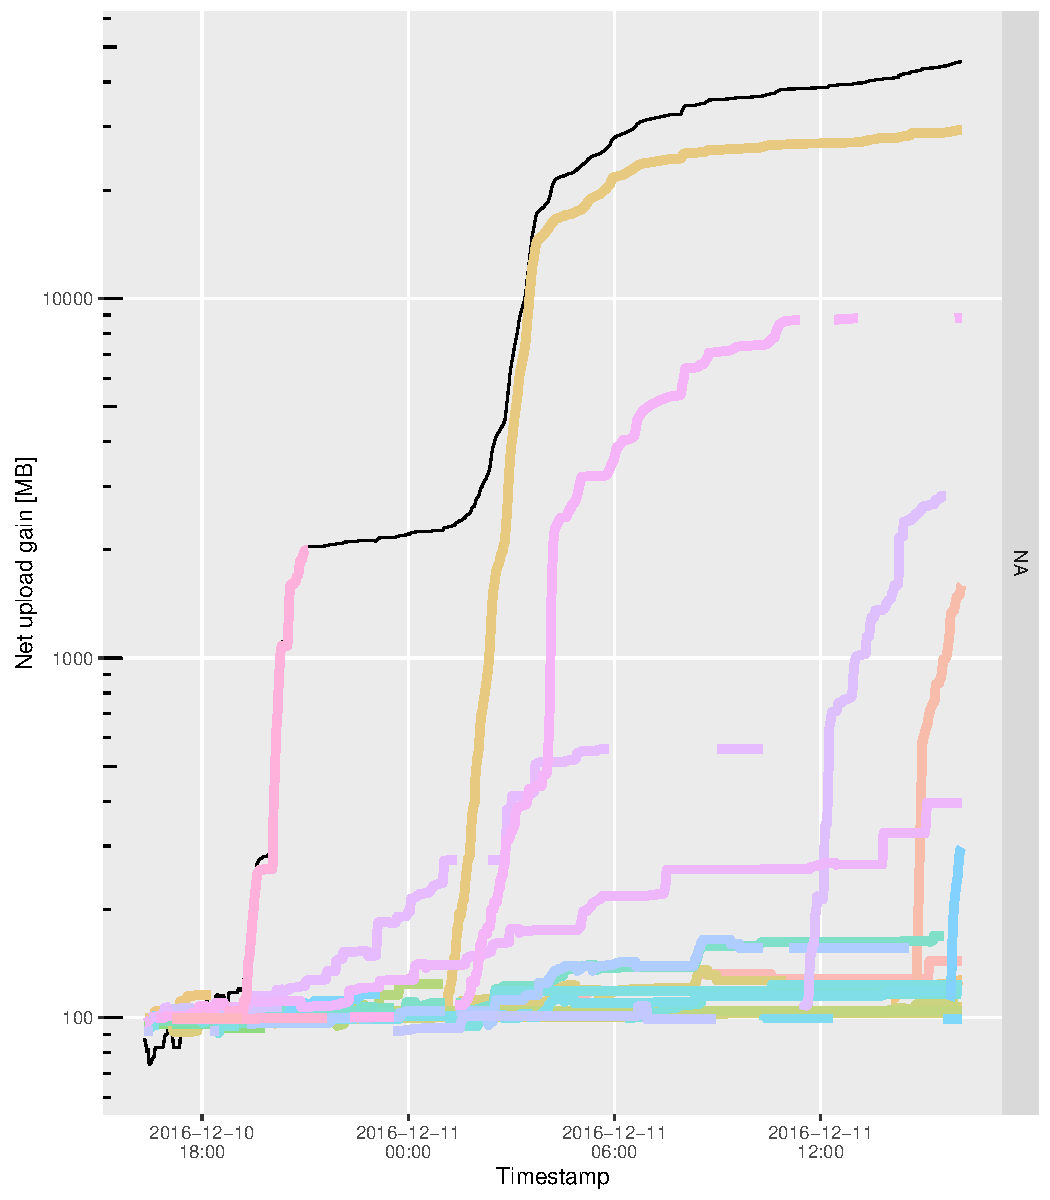
\includegraphics[width=\textwidth]{pics/results/b136.pdf}
			\caption{24 hour new experiment.}
			\label{fig:newetree24}
		\end{subfigure}
		~
		\begin{subfigure}[t]{0.6\textwidth}
			\centering
			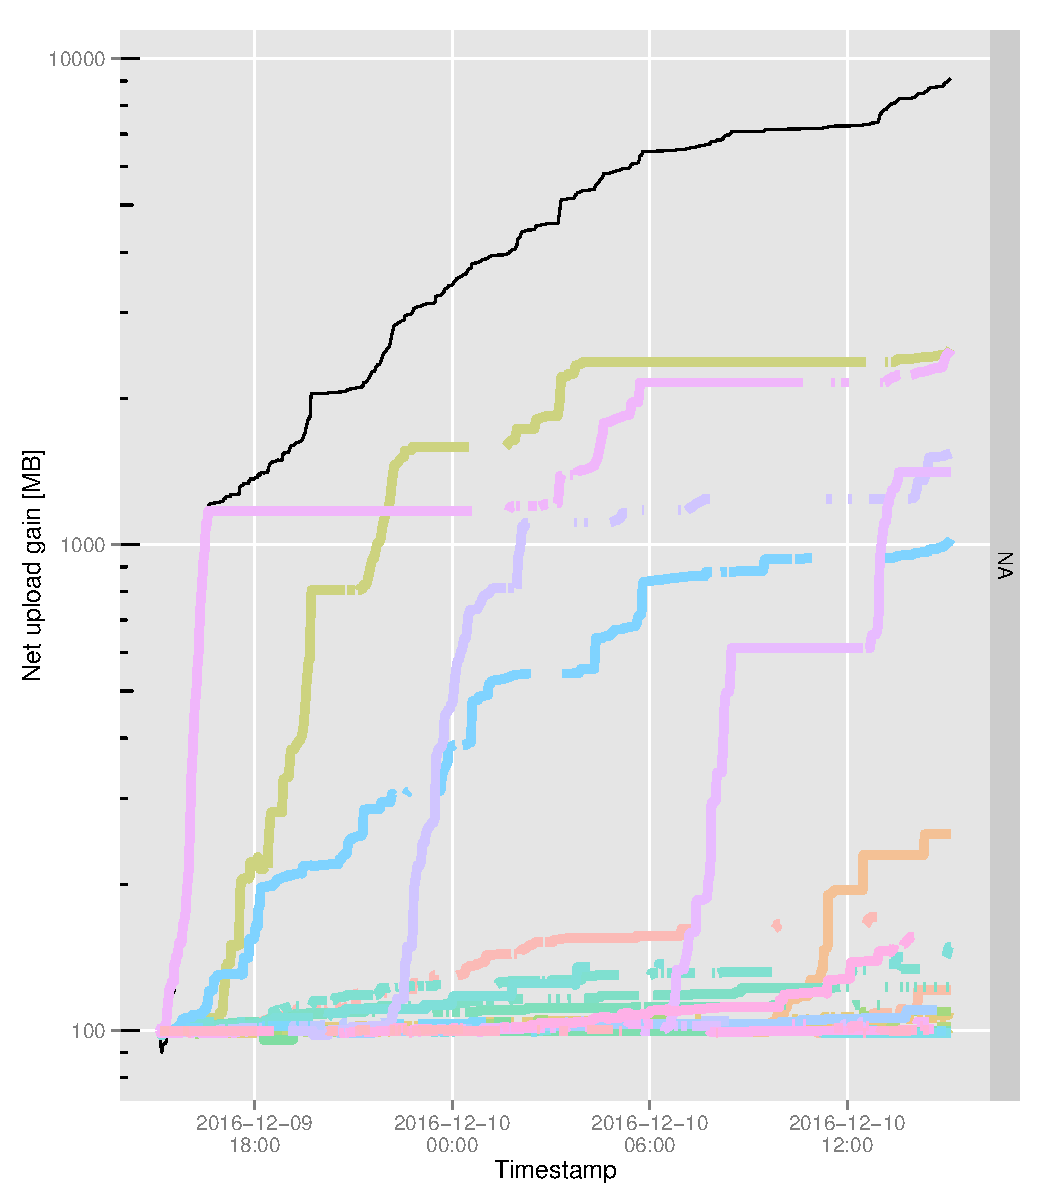
\includegraphics[width=\textwidth]{pics/results/m138.pdf}
			\caption{24 hour old experiment}
			\label{fig:oldetree24}
		\end{subfigure}
		\caption{New vs old experiments (run separately) result on 24 hour (\textit{seederratio} policy)}
	\end{adjustwidth}
\end{figure}
%\todo{re-run with updated code} 
From the figures presented, we can find one similarity. Both of the systems dominated by only a few swarms. It means that not all the recent swarms are popular. Popular swarm means it has more leecher which impacts the overall credit gain. For the main difference, we found two aspects that show new credit mining system is better: policy stability and reducing idleness. In the new system, thanks to investment algorithm, the miners do not need to unnecessarily switch swarm. It shows that the lines tend to more continuous compared to one in prior work. When the line is invisible, it means that particular swarm was not selected in this round. Secondly, it is the idleness of a swarm which is represented in straight horizontal line in the figures. We can successfully reduce the idle swarm by enabling stimulation. In proposed system's experiment, when net upload gained is more than 500 MB, none of the swarm is idle. On the contrary, some swarms in prior work are idle, even when theirs upload gain already high. It can be seen in three straight horizontal line above the 1000 MB gain.

 
\section{Sustaining user experience on downloading}
\label{section:expprio}
As mentioned in \ref{section:uactivityimpl}, credit mining system that implemented within Tribler needs to accommodate user download activity when mining. This experiment will validate that feature. The expectation is that when both credit mining and user download active, the bandwidth used in user download will keep stable. If only credit mining is active, then the system will maximize the bandwidth if possible. 

The experiment runs in the environment as follows. We launched 40 peers and 4 swarms in a single community. One of the swarm contains a file with size 1 GB and rest of the swarms has 2 GB file. Each swarm has 4 dedicated seeders. We then arbitrarily decide the number of downloader for each swarm. All of the peers disabling credit mining except one which we have our interest in. This peer activates credit mining system early without any user download activity. In the middle of the experiment, this peer intentionally downloads a swarm outside the credit mining system. We will then observe our implementation behavior on this event based on the peer's perspective. As for comparison, we launched similar experiment but the peer mentioned above does not activate credit mining system. 

\begin{figure}[h!]
%	\begin{subfigure}[t]{\textwidth}
		\centering
		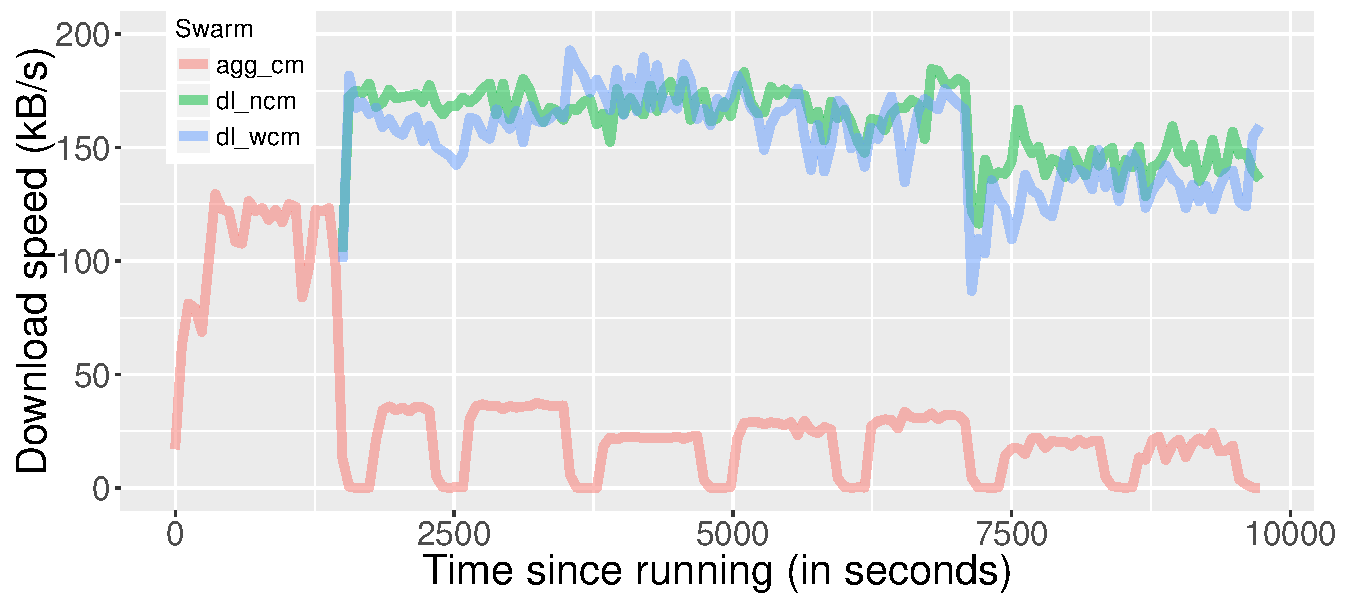
\includegraphics[width=\textwidth]{pics/results/pr_g2-act2.pdf}
		\caption{Download speed of user download activity.}
		\label{fig:cmprio}
\end{figure}

The results in Figure \ref{fig:cmprio} shows the download speed on selected peer with and without activating credit mining. The line which shows user download activity is colored as blue and green. The blue line is run on the experiment with credit mining, while the green line is on the experiment without it. We find that the results match with our expectation regarding bandwidth distribution. Before the new batch of peers arrived to download, both findings resulting similar speed constantly in 150-170 kB/s. After the new batch of peers was coming, the speed can reach up to 150 kB/s for both cases. We conclude that credit mining system has a negligible effect on the overall user experience. 

In Figure \ref{fig:cmprio}, the red line is shown as the accumulative download speed for all the swarm mined. At first, the mining speed is quite high by reaching 125 kB/s. After user promptly downloads a particular swarm, the speed is adjusted to around 45 kB/s. Totaling both mining and downloading activity, it can reach more than 200 kB/s which is 80\% of total download bandwidth. Sometime, the mining speed is 0. This is when the observation phase occurred as elaborated in Section \ref{section:uactivityimpl}. Although not obvious, the general trend of user download and mining speed is contradictory. This can be observable in between time 2500s until 5000s. When the user download speed increase, credit mining system adjusted its mining speed by allocating lower bandwidth. This allocation method also valid on the opposite, which is when the download speed is decreasing. All of these results shows that credit mining system able to run with unused bandwidth. 

\section{Swarm performance with credit mining}
\label{section:swperf}
After we confidently get high return gain from the previous results, it is worth to find out what is the effects of credit mining implementation to the community. The experiment runs with the same setting as from Section \ref{section:evalscoring}, except we add more miners instead of one. We also use scoring policy as default and enable the stimulation. Other parameters are left default. 

Figure \ref{fig:swarmnocmperf} shows the average download speed of all the member in each of the swarm. In this experiment, no credit mining system are active. Some of the swarms have reached its maximum download speed such as \texttt{file1gb\_8}, \texttt{file1gb\_9}, and \texttt{file1gb\_10}. We will take this result as a base figure for the next experiment.

\begin{figure}[h]
	\centering
	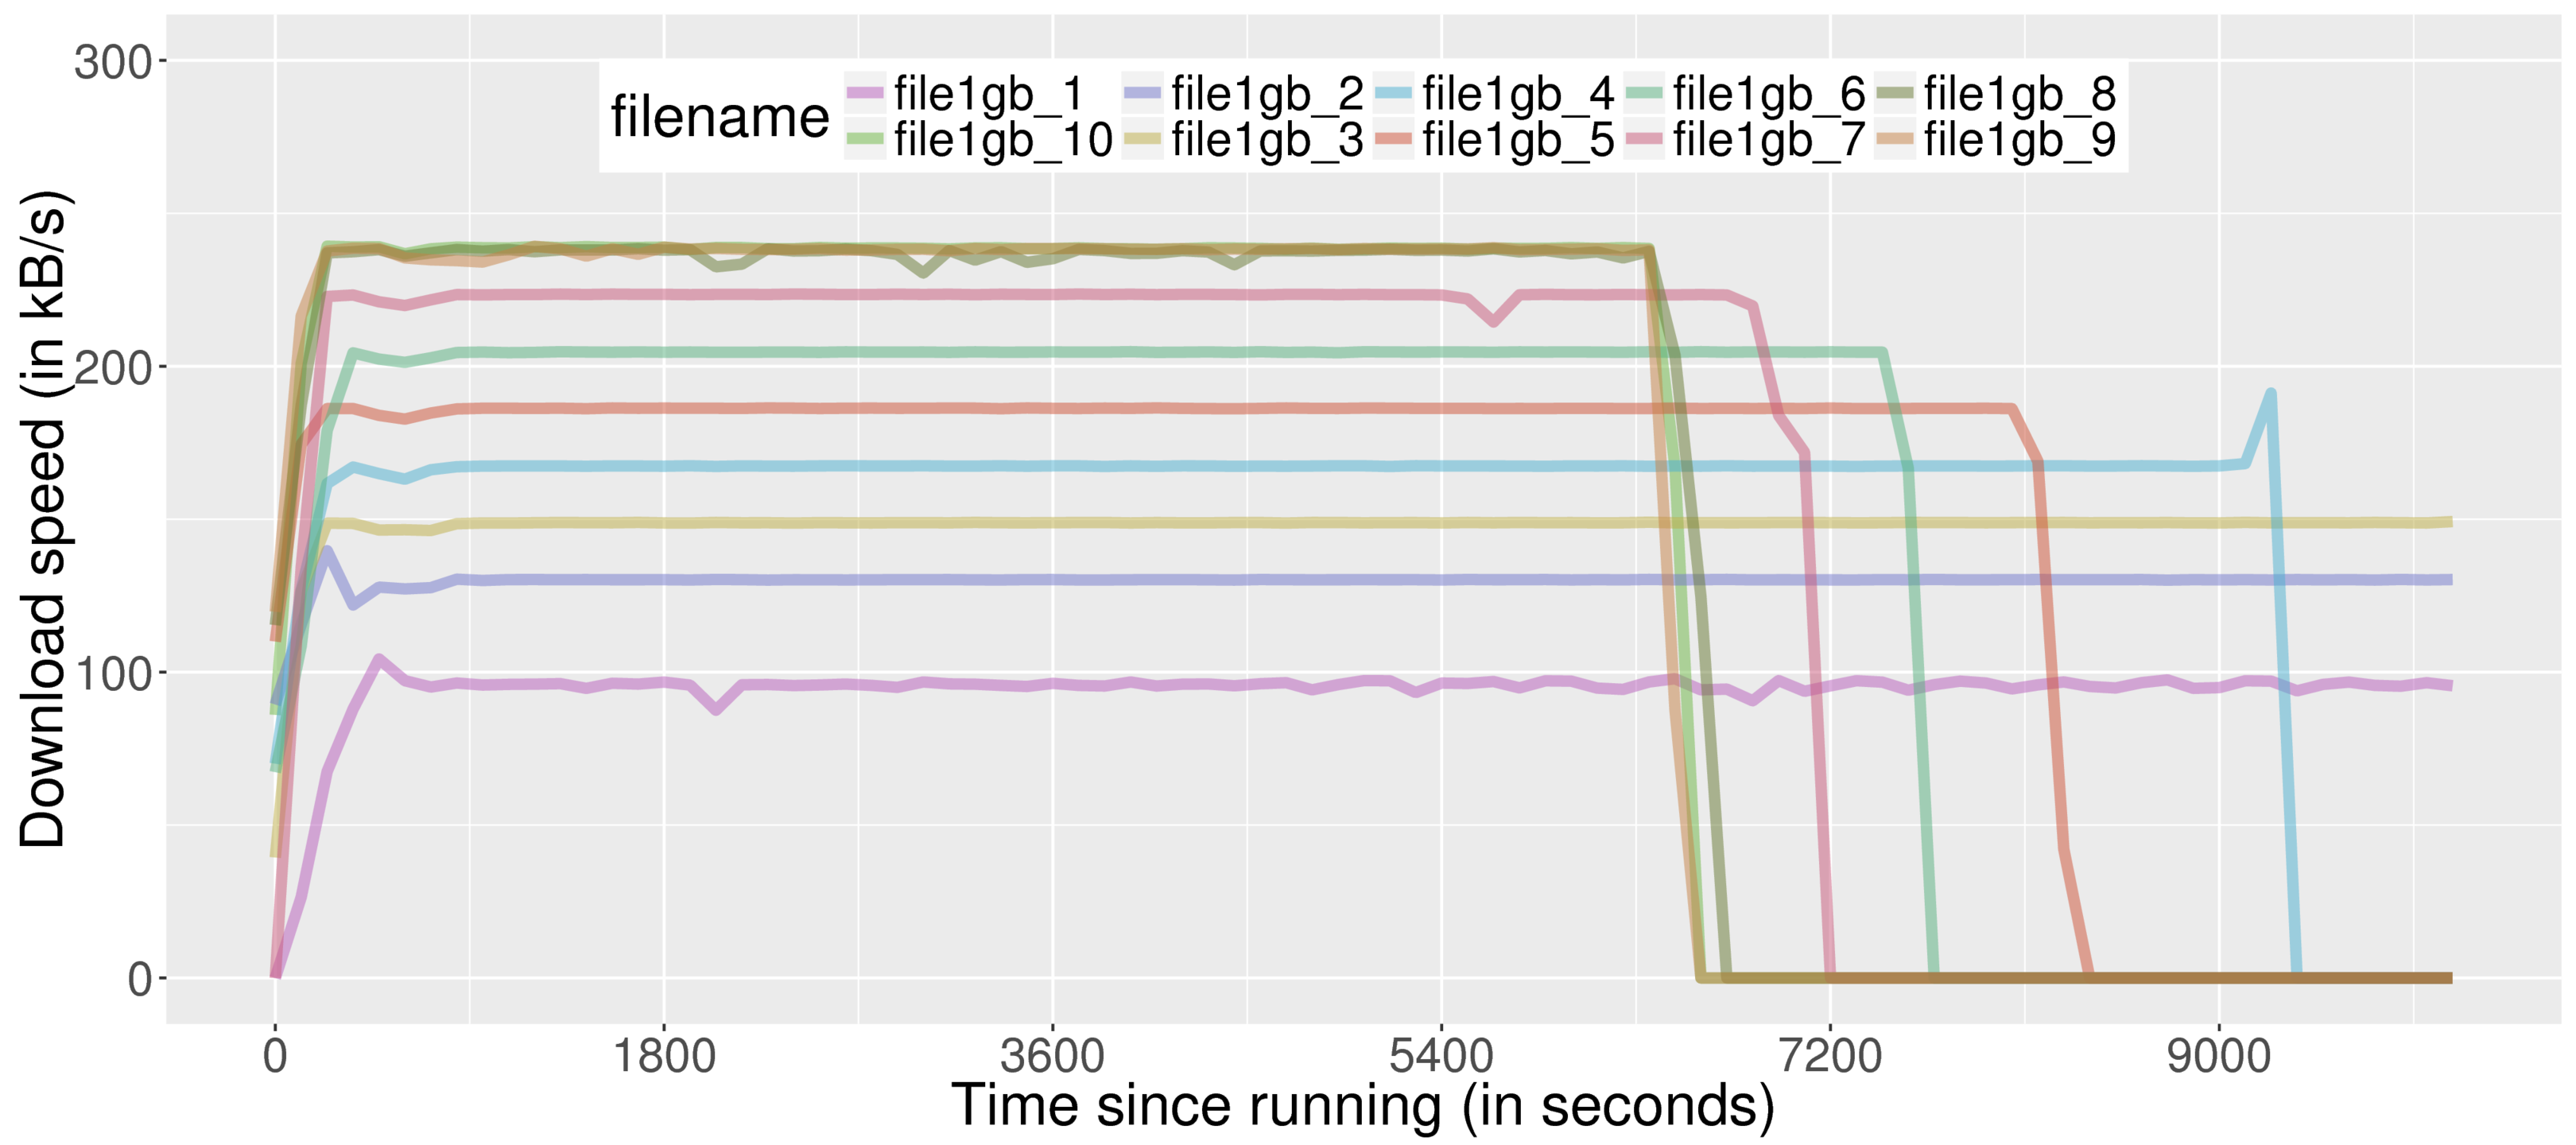
\includegraphics[width=\textwidth]{pics/results/swperf_n2.png}
	\caption{Swarm performance without credit mining}
	\label{fig:swarmnocmperf}
%1   94.57627  exp_3h_swperf_simple_file1gb_1
%4  129.47460  exp_3h_swperf_simple_file1gb_2
%5  147.20364  exp_3h_swperf_simple_file1gb_3
%9  165.74839  exp_3h_swperf_simple_file1gb_4
%3  182.56930  exp_3h_swperf_simple_file1gb_5
%6  199.86998  exp_3h_swperf_simple_file1gb_6
%8  220.01941  exp_3h_swperf_simple_file1gb_7
%10 231.39755  exp_3h_swperf_simple_file1gb_8
%7  232.65703  exp_3h_swperf_simple_file1gb_9
%2  233.83902 exp_3h_swperf_simple_file1gb_10
\end{figure}

%1   exp_3h_swperf_simple_file1gb_1  93.76134  94.57627 -0.8616701
%3   exp_3h_swperf_simple_file1gb_2 168.16871 129.47460 29.8854806
%4   exp_3h_swperf_simple_file1gb_3 185.46871 147.20364 25.9946522
%5   exp_3h_swperf_simple_file1gb_4 196.11774 165.74839 18.3225624
%6   exp_3h_swperf_simple_file1gb_5 218.05894 182.56930 19.4389914
%7   exp_3h_swperf_simple_file1gb_6 210.70760 199.86998  5.4223374
%8   exp_3h_swperf_simple_file1gb_7 221.76209 220.01941  0.7920564
%9   exp_3h_swperf_simple_file1gb_8 232.99379 231.39755  0.6898231
%10  exp_3h_swperf_simple_file1gb_9 231.35478 232.65703 -0.5597267
%2  exp_3h_swperf_simple_file1gb_10 231.79176 233.83902 -0.8754966

Next, we will introduce credit mining system in the swarms. We start by spawning credit mining system half of the number of downloader, which is 25 node. Those are dedicated miners, and all of them started simultaneously. Figure \ref{fig:swarmcm25perf} shows the average download speed from all the downloaders for each of the swarm. We define the swarm is \textit{covered} by credit mining if it significantly (more than 5\%) either get performance increase or drop. In this experiment, the credit mining covers swarm from \texttt{1gb\_2} to \texttt{1gb\_5}. Compared to the previous experiment without credit mining, the download speed is increased from 18.3\% (\texttt{1gb\_4}) to 29.8\% (swarm \texttt{1gb\_2}). For unaffected swarm, the speed can decrease up to 0.8\%.

\begin{figure}[h!]
	\centering
	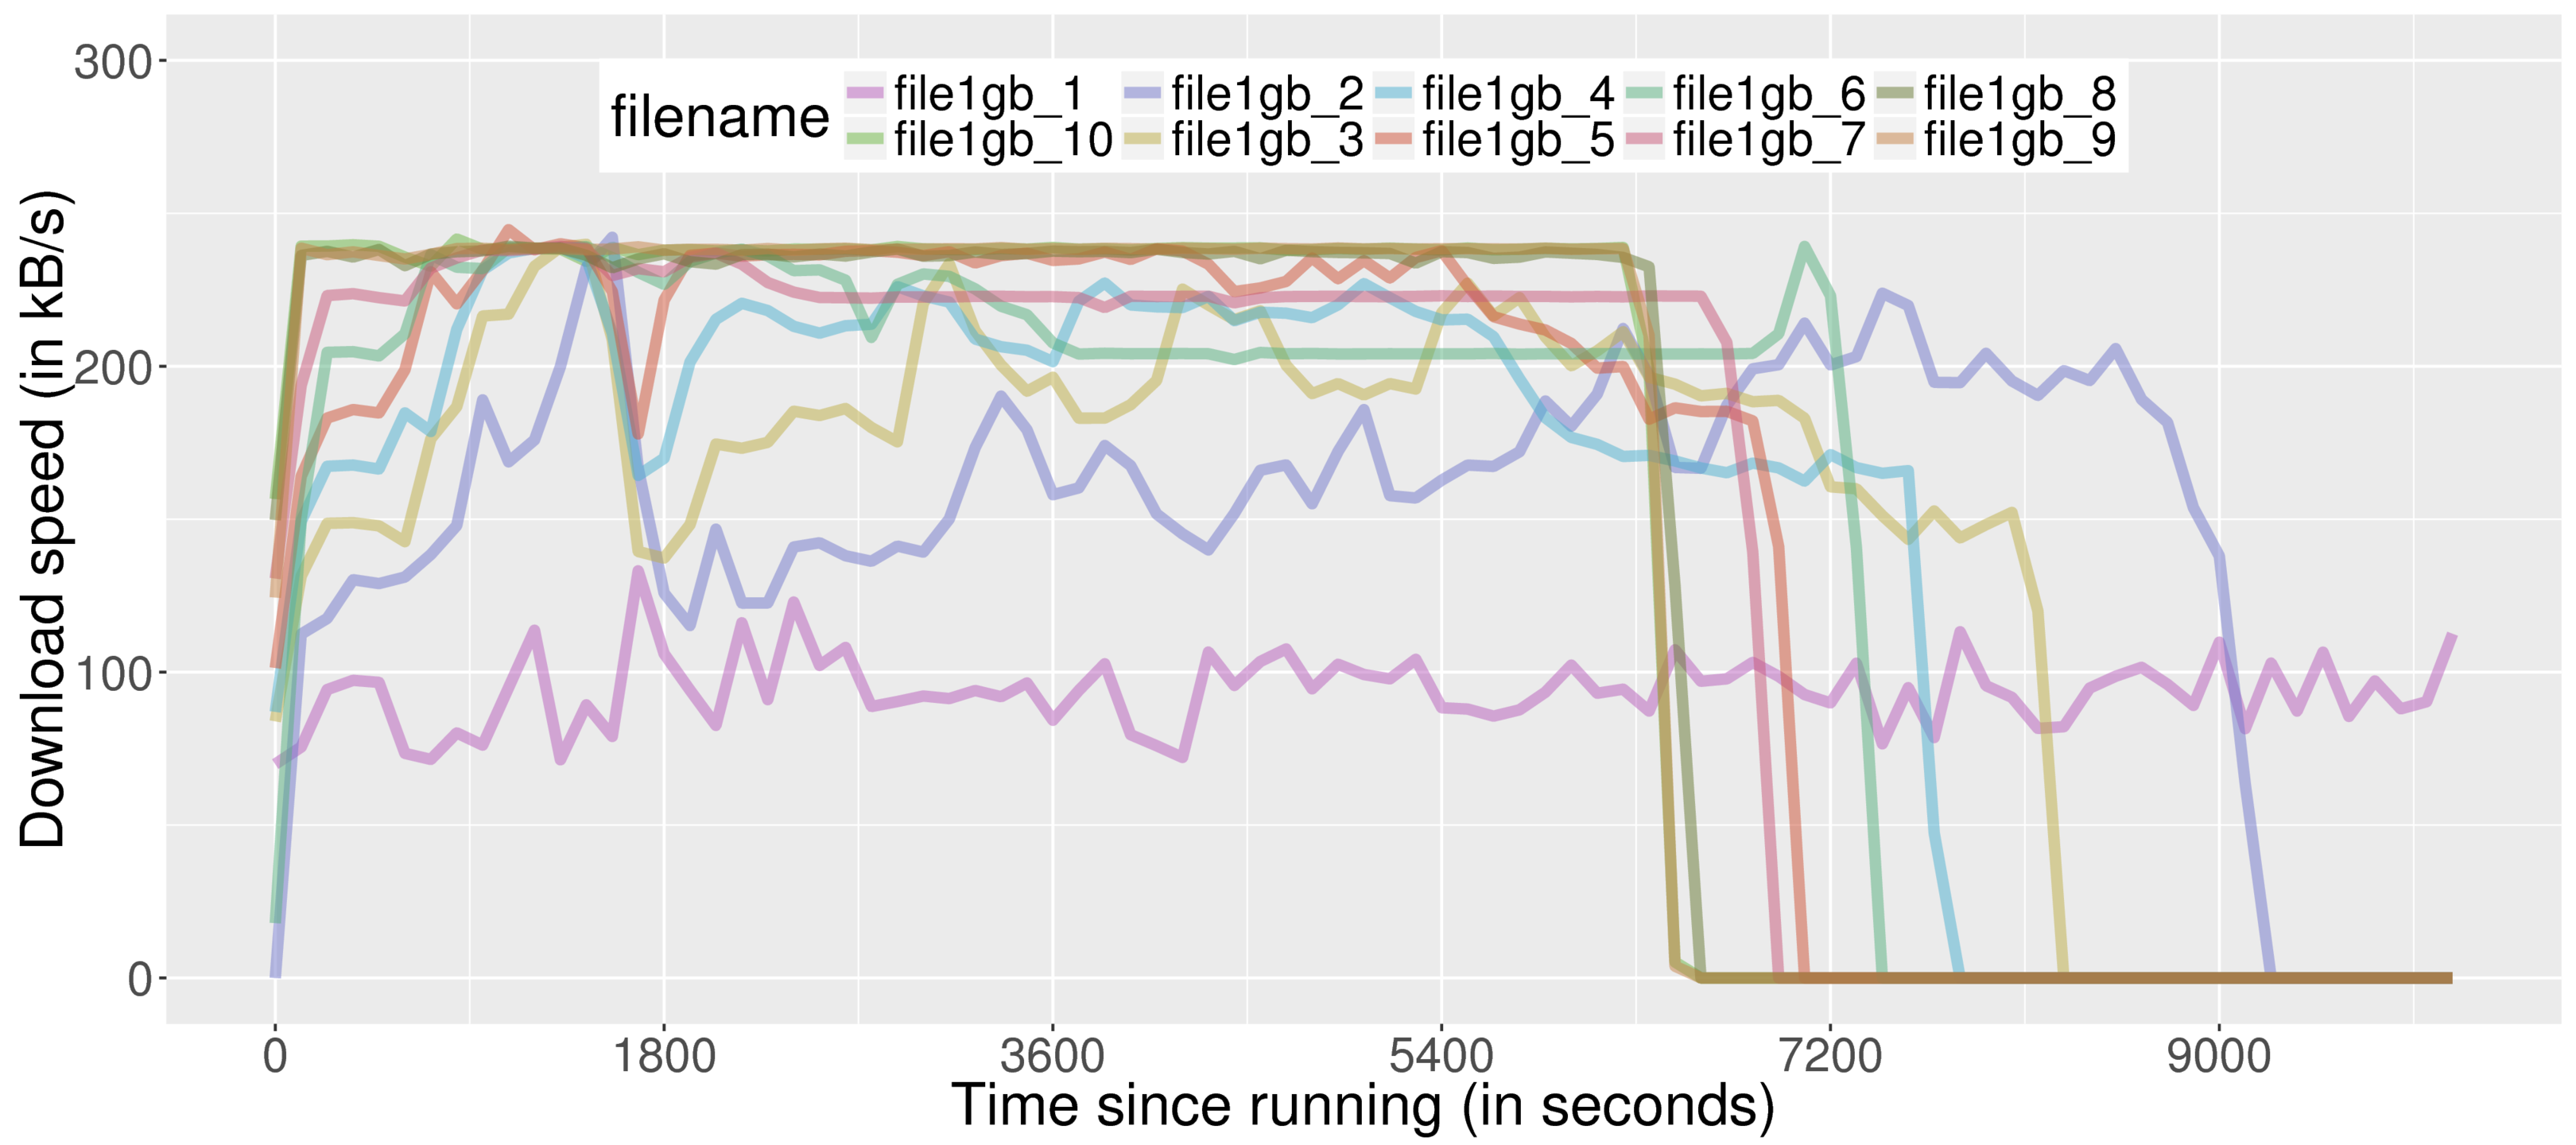
\includegraphics[width=\textwidth]{pics/results/swperf_sc2_25.png}
	\caption{Swarm performance with credit mining in the swarm (25 peers)}
	\label{fig:swarmcm25perf}
	% mean	
	%	1   93.76134  exp_3h_swperf_simple_file1gb_1
	%	4  168.16871  exp_3h_swperf_simple_file1gb_2
	%	5  185.46871  exp_3h_swperf_simple_file1gb_3
	%	9  196.11774  exp_3h_swperf_simple_file1gb_4
	%	3  218.05894  exp_3h_swperf_simple_file1gb_5
	%	6  210.70760  exp_3h_swperf_simple_file1gb_6
	%	8  221.76209  exp_3h_swperf_simple_file1gb_7
	%	10 232.99379  exp_3h_swperf_simple_file1gb_8
	%	7  231.35478  exp_3h_swperf_simple_file1gb_9
	%	2  231.79176 exp_3h_swperf_simple_file1gb_10
\end{figure}

There are two notable drawbacks when introducing credit mining system to the swarm, one of them is that the download speed has become unstable. This exists because of two reasons. First, because of swarm stimulation, there is higher chance for the miners to become more active on downloading pieces. Second, when switching to new swarm, miners has incomplete information on rarest pieces. Therefore, they need to download those pieces to be able to mine. Both reasons have a purpose of maximizing the upload gain as soon as possible. When miner downloads any piece, it took the seeder's bandwidth and then observed speed for other peers looks like decreasing. These factors combined explains the down and up in the Figure \ref{fig:swarmcm25perf}.

The second drawback is the fact that not all the swarms boosted by the system. Swarm with high number of seeders starting from \texttt{1gb\_6} to \texttt{1gb\_10} are not boosted on halfway of the experiment. With the way miners prioritize the swarm, only the lowest-seeded swarm will be filled with miners. In other words, there are not enough miner to boost all the swarm in this experiment. Note that the lowest number of seeder gives worse performance than the base experiment. The reason is that the miner takes seeder's bandwidth that supposed to be downloader's. Therefore, some of the downloaders get the lower speed. However, miners can not give back its downloaded pieces to all downloader. Thus the observed speed is decreasing. In other words, the bottleneck is on the seeder's bandwidth because the seeder can not deliver the piece fast enough for miners to distribute the pieces efficiently.

\subsection{Varying the number of credit miners}
In this experiment, we will change the number of credit miners in a swarm. First, we double it to 50 nodes. The average download speed observed from peers can be seen in Figure \ref{fig:swarmcmperf}. Although the download instability is still there, not only the speed is faster than the previous experiment with 25 miners but also it overcomes the second drawback. Compared to the previous experiment, this shows that the number of miners relates to the boosting coverage of swarms. With 50 miners, it is enough to cover all the possible swarm in this environment. The exceptional case on swarm with single seeder still hold. Moreover, with 50 swarms, it can increase the swarm's download speed up to 34.6\% (swarm \texttt{1gb\_3}). The lowest increasing performance is on swarm \texttt{1gb\_7} with 3.9\%. The average increase for the covered swarm is 17.98\%.

\begin{figure}[h]
	\begin{subfigure}[h]{\textwidth}
		\centering
		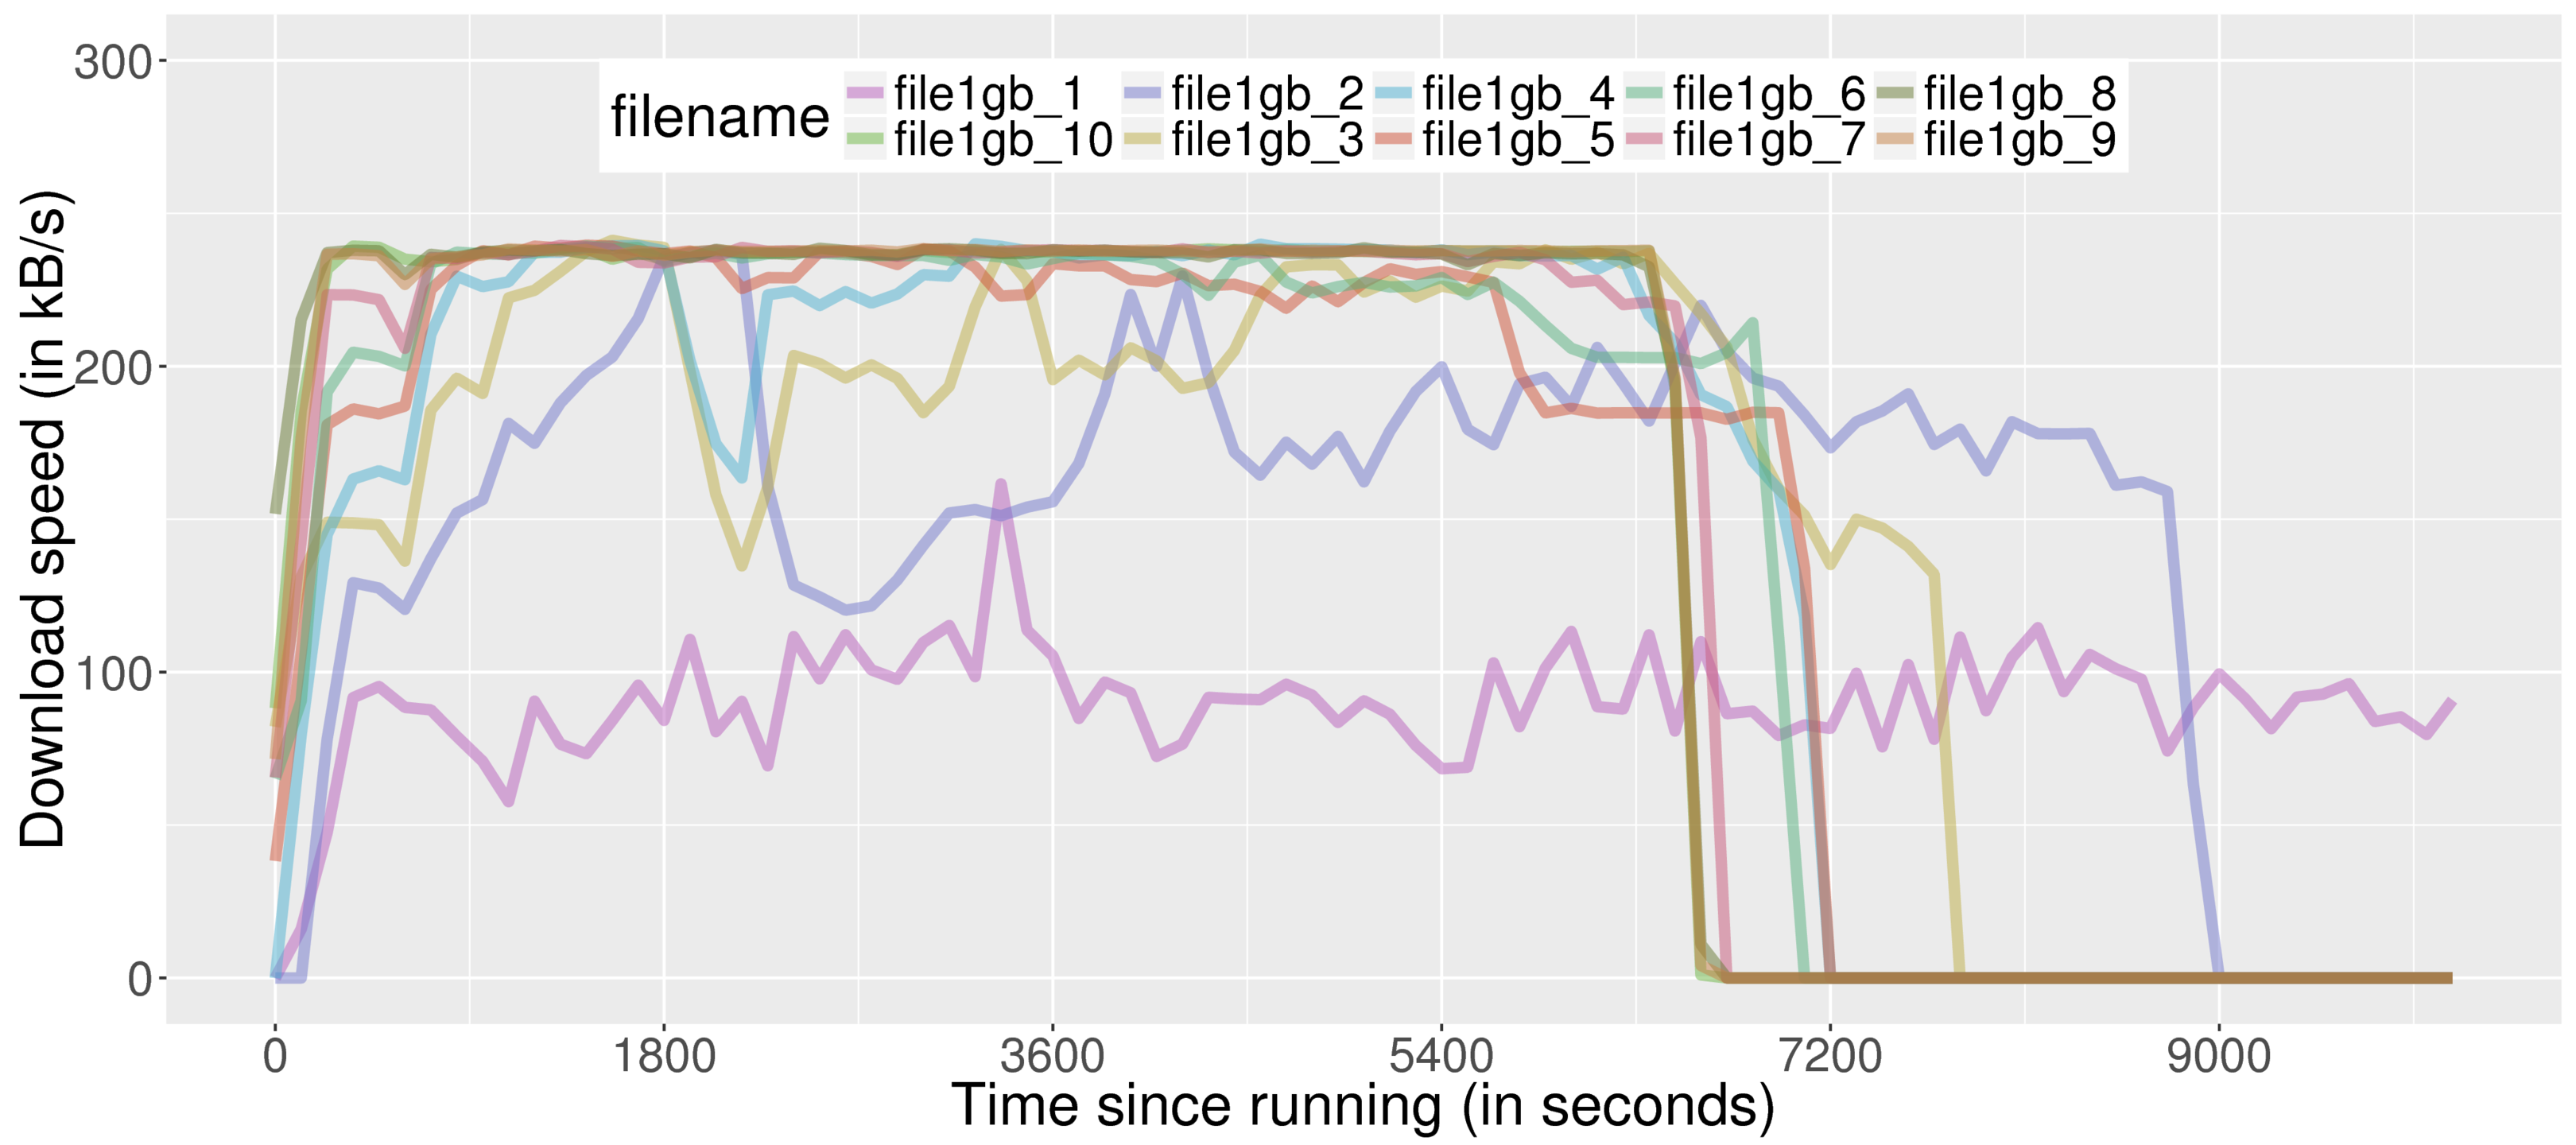
\includegraphics[width=\textwidth]{pics/results/swperf_sc2.png}
		\caption{Swarm performance with credit mining in the swarm (50 peers)}
		\label{fig:swarmcmperf}
		%		1   90.44611  exp_3h_swperf_simple_file1gb_1 -4.36701510854678
		%		4  174.32050  exp_3h_swperf_simple_file1gb_2 34.6368322435443
		%		5  197.69961  exp_3h_swperf_simple_file1gb_3 34.3034791802702
		%		9  216.80348  exp_3h_swperf_simple_file1gb_4 30.8027667719729
		%		3  213.11578  exp_3h_swperf_simple_file1gb_5 16.7314438955509
		%		6  219.55919  exp_3h_swperf_simple_file1gb_6 9.8510091410426
		%		8  228.68752  exp_3h_swperf_simple_file1gb_7 3.93970241080095
		%		10 230.21745  exp_3h_swperf_simple_file1gb_8 -0.509988113530142
		%		7  228.38337  exp_3h_swperf_simple_file1gb_9 -1.83689269995409
		%		2  228.60623 exp_3h_swperf_simple_file1gb_10 -2.23777451684496
		
	\end{subfigure}
	\begin{subfigure}[h]{\textwidth}
		\centering
		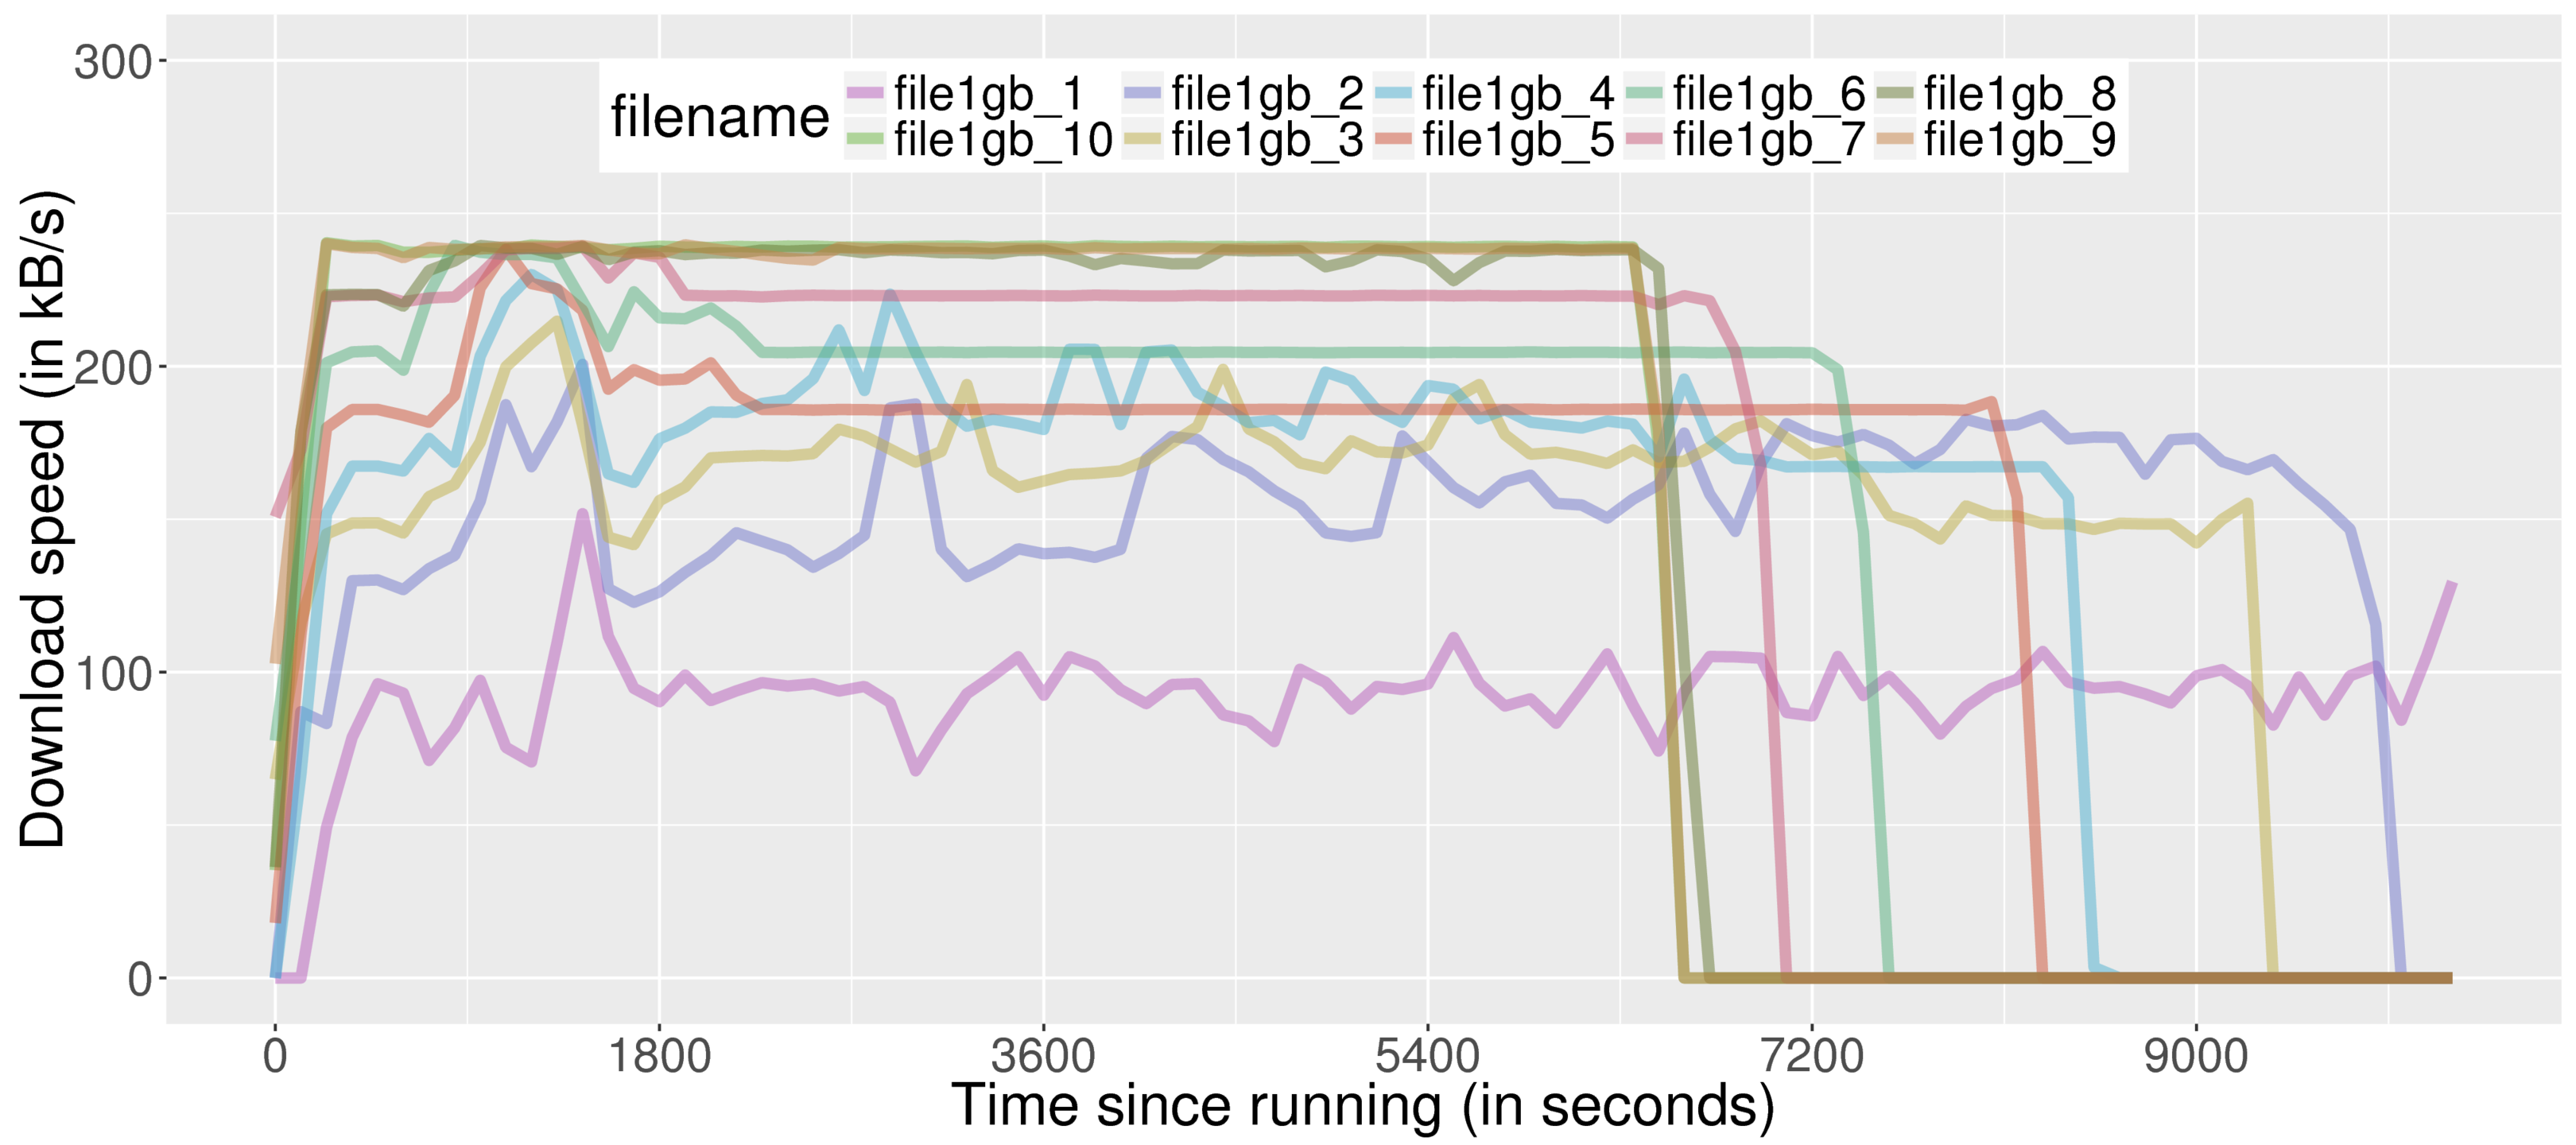
\includegraphics[width=\textwidth]{pics/results/swperf_sc1_10.png}
		\caption{Swarm performance with credit mining in the swarm (10 peers)}
		\label{fig:swarmcm10perf}
	\end{subfigure}
	%	          average_speed   filename 
	%	          1   93.84661  file1gb_1	
	%	          4  156.09825  file1gb_2
	%	          5  165.20124  file1gb_3
	%	          9  179.36101  file1gb_4
	%	          3  185.69509  file1gb_5
	%	          6  204.56280  file1gb_6
	%	          8  221.31673  file1gb_7
	%	          10 228.48779  file1gb_8
	%	          7  233.63073  file1gb_9
	%	          2  232.48323  file1gb_10
	\caption{The effect of different number of miners on swarm.}
\end{figure}

Second, we also conducted an experiment with less number of miners. In this case, the number of credit miners in the swarm is set to 10 nodes. From Figure \ref{fig:swarmcm10perf}, it is shown that the coverage is lessened. Now, half of the swarms (from \texttt{1gb\_5} to \texttt{1gb\_10}) are not boosted by the miners. The average speed is slightly higher compared to base experiment but lower than 25-miners experiment. The highest performance increase is on swarm \texttt{1gb\_2} with 20.5\%, and the lowest is on \texttt{1gb\_4} with 8.21\%.


\subsection{The effect of swarm stimulation}
\begin{figure}[h!]
	\centering
	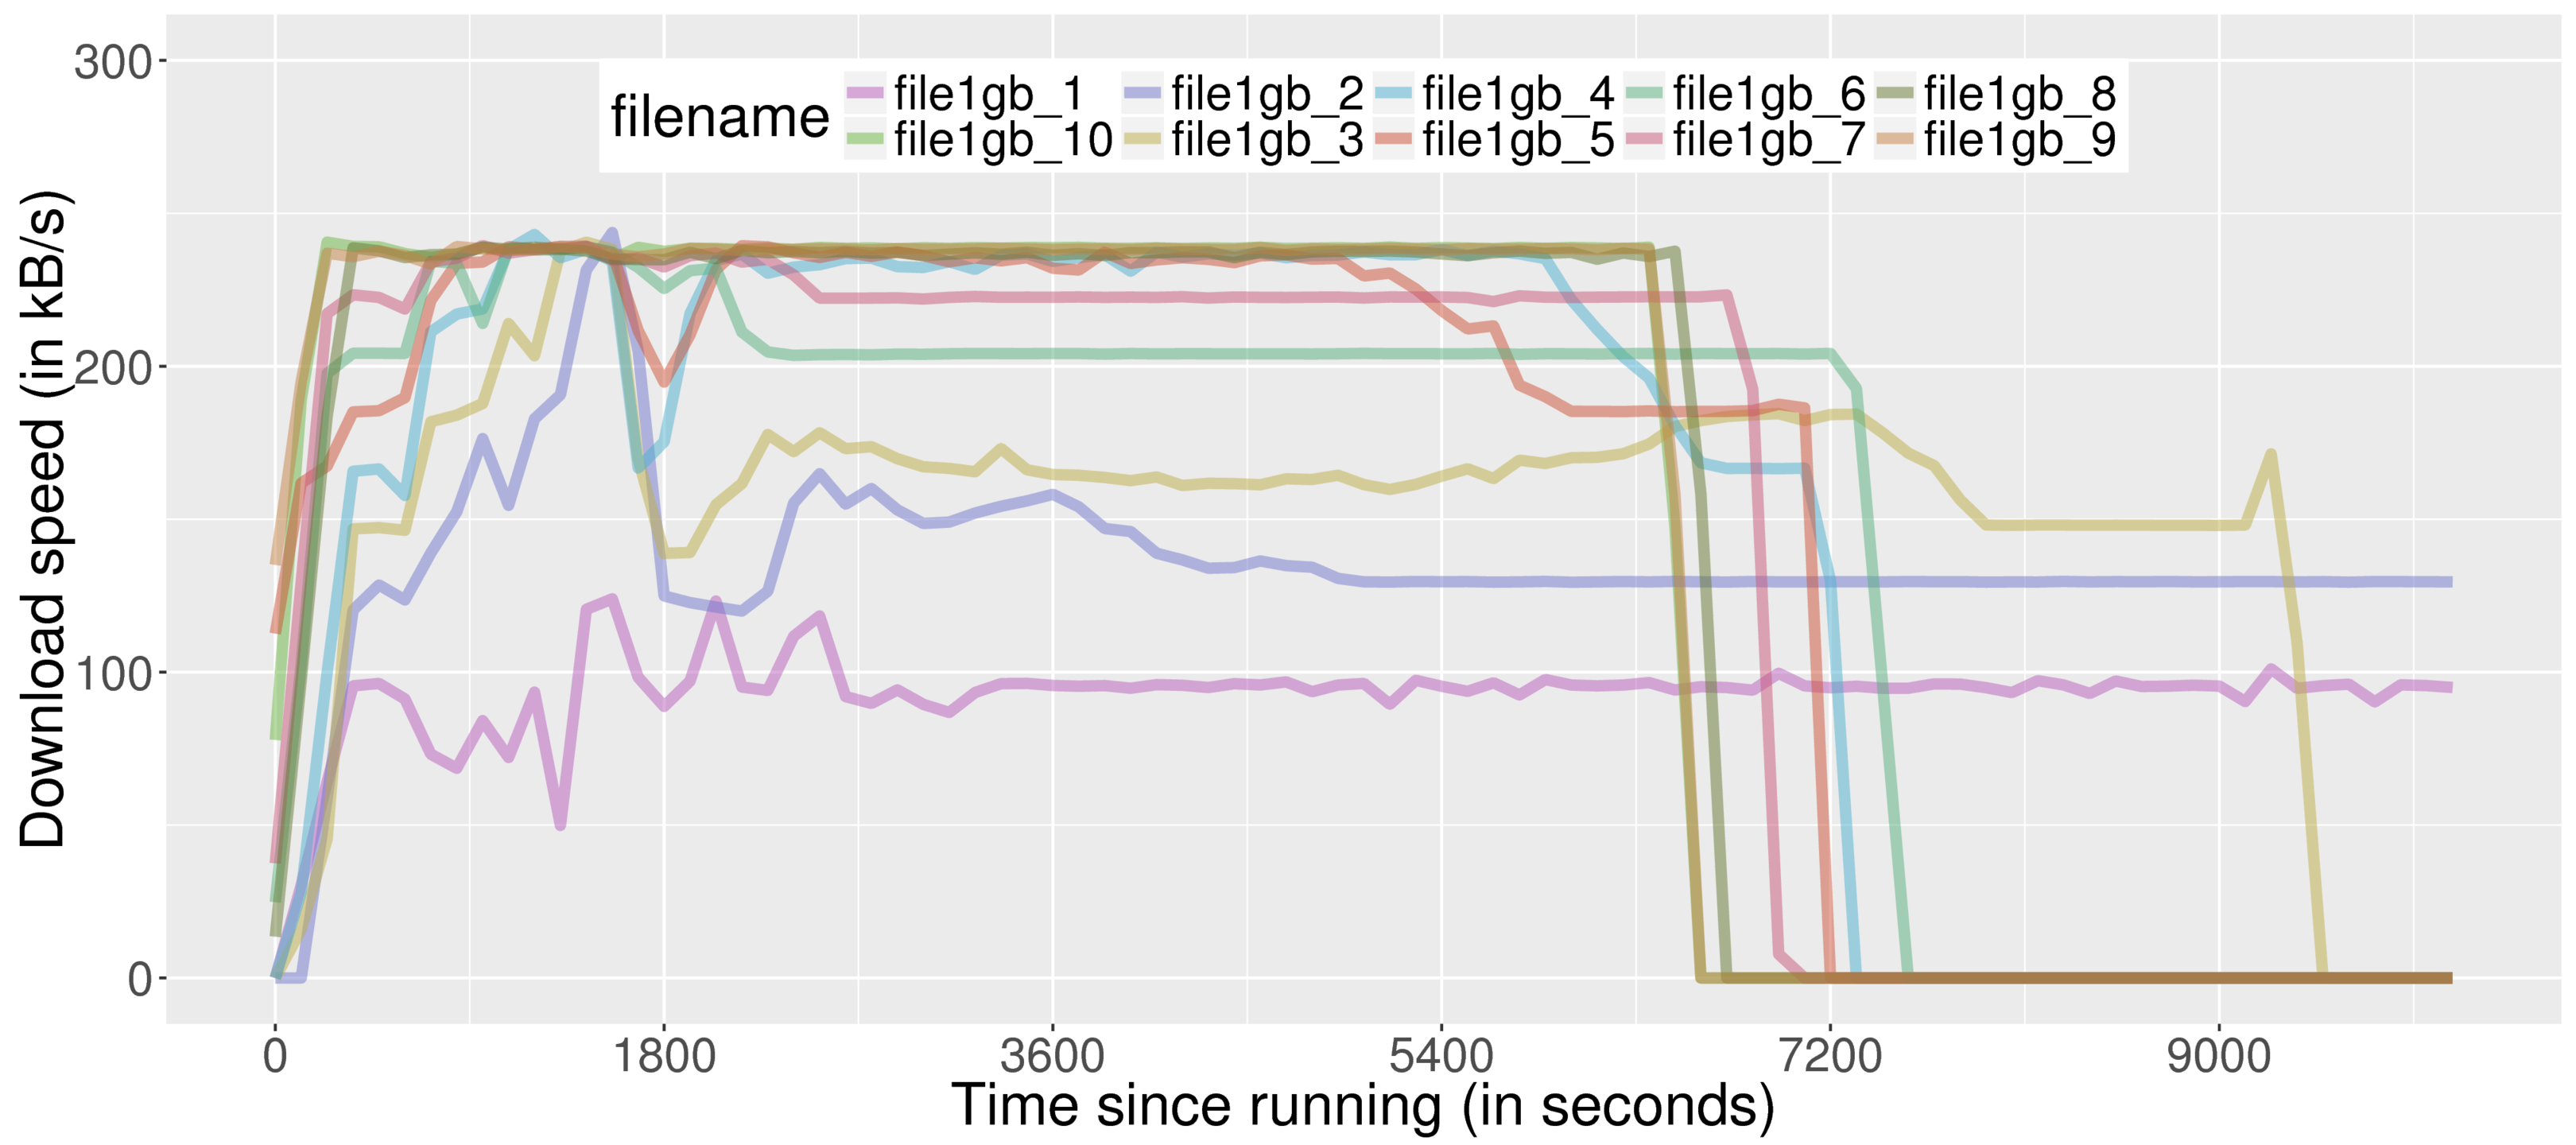
\includegraphics[width=\textwidth]{pics/results/swperf_sc1_notrig.png}
	\caption{Swarm performance with credit mining in the swarm (25 peers) without stimulation.}
	\label{fig:swarmcm25perfnotrig}
	%		avg_dl_speed fname
	%	1   93.68527  file1gb_1
	%	4  138.86226  file1gb_2
	%	5  164.62305  file1gb_3
	%	9  212.60381  file1gb_4
	%	3  215.89967  file1gb_5
	%	6  203.22903  file1gb_6
	%	8  216.89871  file1gb_7
	%	10 228.13082  file1gb_8
	%	7  233.89741  file1gb_9
	%	2  232.99496 file1gb_10
\end{figure}

Our next experiment is to understand the effect of swarm stimulation to the community. As shown before (Section \ref{section:resultgain}), swarm stimulation can increase credit gain for the user. A notable difference from this experiment is that the average speed instability is gone as can be seen in Figure \ref{fig:swarmcm25perfnotrig}. However, as a trade-off, the average speed is slightly lower on boosted swarm. Compared to experiment with 25 miners, only swarm \texttt{1gb\_4} is better with 8\% increased download speed. The rest have their performance decreased starting from 1\% (\texttt{file1gb\_5}) to 17\% (\texttt{file1gb\_2}) . However, it is still better than the base experiment. Swarm \texttt{file1gb\_4} improves as much as 28\% and swarm \texttt{file1gb\_2}, despite has the worst decreasing performance compared to one with 25-miners, still improves by 7.25\%. Other disadvantages are on the lower-seeded swarm, namely \texttt{1gb\_1} and \texttt{1gb\_2}, it has negligible difference with base experiment, especially in the latter half of the experiment. Therefore, the coverage of boosted swarm is also reduced. 

When swarm stimulation is enabled, it will consume the bandwidth from both seeder and downloader if necessary. After it finished downloading rarest pieces, it immediately returns the bandwidth it consumed back to the community in equal or higher amount. That explains the bumps which represented instability of the downloaders' download speed. However, we argue that stimulate swarm with very few seeder is counterproductive. Although the stimulation can widely be enabled on all the swarm which gives very little drawback, it seems is not suitable for some swarms. 

